\documentclass[10pt]{book}

\usepackage{cdt/cdtUsecases}
\usepackage{txfonts}


% !TeX root = proyecto.tex

% Encabezados y pie de página
\fancyhead[LE]{
\includegraphics[height=35pt]{theme/headerPar}} 
\fancyhead[RO]{
\includegraphics[height=35pt]{theme/headerInp}} 
\fancyhead[RE]{} 
\fancyhead[LO]{} 

\fancyfoot[CO,CE]{{\tiny\color{subTitleColor}\em Av. Juan de Dios Bátiz esq. Miguel Othón de Mendizabal S/N Col. Lindavista, GAM, D. F. {\color{sectionColor}\Telefon} 57296000 Ext. 52004 {\color{sectionColor}\Letter} ulises.velez@gmail.com}}
\fancyfoot[RO,LE]{\footnotesize\thepage}


%=========================================================
% Datos del documento:
\defProyecto{Sistema de Gestion Escolar PRONIM}
\defNumComponente{Componente 2}
\defComponente{Documento de análisis}
\defEtapa{Etapa del documento: iteración 3}

%=========================================================
% Datos de la consultora:
\defConsultora{KAVA}
\defNomSupervisor{Nombre del responsable por parte de la consultora}
\defCargoSupervisor{Cargo del responsable de la consultora: Líder de proyecto, Scrum Master, Project Manager, etc.}

%=========================================================
% Datos del cliente:
\defCliente{Dirección General de Desarrollo de la Gestión e Innovación
Educativa}
\defNomResponsable{Nombre del responsable del proyecto por parte de la empresa}
\defCargoResponsable{Cargo del responsable de la empresa}

\setlength{\parskip}{10pt} % Pone un espacio entre párrafos de 10 puntos

\title{\Proyecto\bigskip\\\Componente}
\subtitle{\Etapa}
\author{\Consultora}
\organization{\Cliente}
\showInstrucciones
\date{\color{green}\today}

%%%%%%%%%%%%%%%%%%%%%%%%%%%%%%%%%%%%%%%%%%%%%%%%%%%%%%%%%%%%%%%%

\begin{document}
\renewcommand{\listtablename}{Índice de tablas}
\renewcommand{\tablename}{Tabla} 
\ThisLRCornerWallPaper{1}{theme/bannerAzul}
\maketitle
\thispagestyle{empty}

\frontmatter
\tableofcontents
\listoffigures
\listoftables

% !TeX root = proyecto.tex

%=========================================================
%\chapter{Project Charter}

\newcommand{\ESCOMPchSec}[1]{\rowcolor{colorAgua}\multicolumn{4}{|c|}{\bf #1}\\\hline}
\newcommand{\ESCOMPchItem}[2]{{\bf {#1}} & \multicolumn{3}{p{.66\textwidth}|}{#2}\\\hline}
\newcommand{\ESCOMPchSubItem}[3]{{\bf {#1}} & {#2} & \multicolumn{2}{p{.44\textwidth}|}{#3}\\\hline}
\newcommand{\ESCOMPchSubSubItem}[4]{{\bf {#1}} & {#2} & {#3}& {#4}\\\hline}

\cleardoublepage
{\centering{\Huge Project Charter}\bigskip\\}
\begin{table}[hptb!] 
%\renewcommand\thetable{i}
\begin{tabular}{|p{.22\textwidth} |p{.22\textwidth} |p{.22\textwidth} |p{.22\textwidth} |}
	\hline
	\ESCOMPchItem{Proyecto:}{CVE, Nombre proyecto.}
	\ESCOMPchItem{Responsable:}{Empresa, Nombre del responsable, cargo, Firma.}
	\ESCOMPchItem{Autoriza:}{Empresa, Nombre del responsable, cargo, Firma.}
	\ESCOMPchItem{Background/Contexto:}{Descripción breve del contexto, no mas de 3 líneas.}
	\ESCOMPchItem{Beneficios esperados:}{Principales beneficios al término del proyecto.}
	\ESCOMPchItem{Costo estimado:}{\$ 2,350,700.00 $\pm$ 13\% (por ejemplo.)}
	\ESCOMPchSubSubItem{Fecha de inicio:}{Fecha}{\bf Fecha de término:}{Fecha.}
	\ESCOMPchItem{Objetivo:}{Objetivo general del proyecto.}
	\ESCOMPchSec{Entregables Principales}
	\ESCOMPchSubItem{}{Clave-Nombre}{descripción del entregable}
	\ESCOMPchSubItem{}{Clave-Nombre}{descripción del entregable}
	\ESCOMPchSubItem{}{...}{}
	\ESCOMPchSec{Alcance del proyecto}
	\ESCOMPchItem{Incluye:}{
		\begin{Titemize}
			\Titem Elemento 1 del alcance que incluye.
			\Titem ...
		\end{Titemize}
	}
	\ESCOMPchItem{Excluye:}{
		\begin{Titemize}
			\Titem Elemento 1 del alcance que incluye.
			\Titem ...
		\end{Titemize}
	}
	\ESCOMPchItem{Criterio de éxito:}{Indicador clave de término del proyecto}
	\ESCOMPchItem{Metodología:}{Metodología o metodologías que se utilizan (dos renglones o lista de no mas de 7)}
	\ESCOMPchSec{Datos de contacto}
	\ESCOMPchItem{Project Manager:}{Nombre, Tel, correo, etc.}
	\ESCOMPchItem{Project owner:}{Nombre, Tel, correo, etc.}
	\ESCOMPchItem{...}{}
	\ESCOMPchItem{Riesgos y peligros:}{
		\begin{Titemize}
			\Titem Riesgo o peligro identificado.
			\Titem ...
		\end{Titemize}
	}
	\ESCOMPchItem{Supuestos:}{
		\begin{Titemize}
			\Titem Suposiciones hechas de las que depende el éxito del proyecto.
			\Titem ...
		\end{Titemize}
	}
	\ESCOMPchItem{Restricciones y dependencias:}{
		\begin{Titemize}
			\Titem Restricciones del proyecto.
			\Titem ...
		\end{Titemize}
	}
	\ESCOMPchSec{Supervisión}
	\ESCOMPchSubItem{Juntas:}{(Nombre de la(s) persona(s)),}{ reporta a (Nombre de la(s) persona(s))}
	\ESCOMPchSubItem{Dudas:}{(Nombre de la(s) persona(s)),}{ reporta a (Nombre de la(s) persona(s))}
	\ESCOMPchSubItem{Avances:}{(Nombre de la(s) persona(s)),}{ reporta a (Nombre de la(s) persona(s))}
	\ESCOMPchSubItem{...}{}{}
\end{tabular}
	\caption{Resumen del proyecto}
	\label{tbl:projectCharter}
\end{table}


\mainmatter % Inicio del contenido contenido principal (numeración
\LRCornerWallPaper{1}{theme/pleca} % Coloca la imagen de la pleca en la esquina inferior derecha

%%%%%%%%%%%%%%%%%%%%%%%%%%%%%%%%%%%%%%%%%%%%%%%%%%%%%%%%%%%%%%%%

%=========================================================
% !TeX root = proyecto.tex

%=========================================================
\chapter{Introducción}


\cdtInstrucciones{
	Presentar el documento, indicando su contenido, a quien va dirigido, quien lo realizó, por que razón, dónde y cuando. \\
}
	Este documento contiene el análisis de requerimientos del proyecto ``{\em Nombre del proyecto}'' que servirá como base para el análisis, diseño, construcción, pruebas y aceptación del proyecto.

%---------------------------------------------------------
\section{Presentación}


\cdtInstrucciones{
	Presente en un par de párrafos el contexto y el problema en que se define el proytecto.
}
El Programa de Educación Básica para Niños y Niñas de Familias Jornaleras Agrícolas Migrantes (PRONIM) brinda atención educativa a niñas y niños de familias jornaleras agrícolas migrantes y/o asentadas, de 3 a 16 años de edad. Opera en los centros educativos ubicados en las comunidades y en los campamentos agrícolas de destino de esta población, en ellos brindan las condiciones para que con la participación de docentes, asesores escolares, asesores técnico-pedagógicos, se lleve a cabo una atención educativa de calidad.
Sin embargo la movilidad entre los distintos Centros de Trabajo que estan acobijados dentro del PRONIM es complicada de realizar debido a la falta de comunicación entre los distintos Centros de Trabajo, este pequeño problema genera grandes afectaciones al desarrollo de los niños y niñas registradas en el programa.

\cdtInstrucciones{
	Indique el propósito del documento, a quien va dirigido y como debe ser utilizado el documento.
}\\
El proposito del presente documento es mantener la comunicación entre los miembros del equipo de desarrollo además de generar los acuerdos necesarios para la aceptación del mismo, este documento debe ser actualizado para mantener su correcto funcionamiento. 
%---------------------------------------------------------
\section{Organización del contenido}

\cdtInstrucciones{
	Indique el contenido y organización del documento.
}\\
	En el capítulo \ref{cap:alcance} podemos encontrar la información relativa al alcance propuesto para este proyecto que incluye el analisis de la problematica, problemas identificados,contexto, analisis de las causas y consecuencias, caracteristicas y sintesis de la solución, asi como los objetivos del proyecto, los usuarios del sistema, procesos que se veran afectados por la adopción del sistema, requerimientos del usuario y la especificación de la plataforma.
	
	En el capítulo \ref{cap:reqSist} ...

%---------------------------------------------------------
\section{Notación, símbolos y convenciones utilizadas}

\cdtInstrucciones{
	Indique la notacion utilizada así como nórmas o estándares de documentación utilizados en el documento.
}	
Todos los diagramas incluidos en este documento que sean posible modelar bajo el marco de UML seran modelados con base en sus normas.
Los terminos especificos para el negocio seran descritos en \ref{sec:terminosDeNegocio}


%=========================================================
% !TeX root = proyecto.tex

%=========================================================
\chapter{Modelo del alcance}
\label{cap:alcance}

\cdtInstrucciones{
	Indique un resumen que describa el contenido del capítulo.
}
	En este capítulo, exploraremos el objetivo del proyecto, junto con las limitaciones que determinan el alcance del mismo. Añadido a eso definiremos a los usuarios involucrados en el sistema, sus roles y las plataformas compatibles en las que se desarrollará e implementará el proyecto. Nos enfocaremos en identificar las problemáticas clave, desglosando las causas que probablemente las originan y evaluando las consecuencias más probables que podrían surgir si no se abordan adecuadamente.

Asimismo, presentaremos posibles soluciones para cada uno de los problemas detectados, con una síntesis final que propondrá una solución integral capaz de satisfacer la mayor cantidad de requerimientos de los usuarios. Detallaremos los requisitos específicos de los usuarios, ya que serán fundamentales para guiar el diseño y el desarrollo del proyecto en todas sus etapas posteriores, asegurando que se cumplan sus expectativas y necesidades.
%---------------------------------------------------------
\section{Análisis de la problemática}

\cdtInstrucciones{
	Indique en un párrafo o dos el contenido y organización de la problemática.
}
Durante el proceso de migarción al que se ven sometidos los niños inscritos en el PRONIM gran parte de la información necesaria para determinar su nivel educativo se ve retrasada o nunca llega a ser proporcionada al centro de trabajo en el que el niño se va  a incorporar, esto puede ocasionarle un retraso en el desarrollo de las habilidades necesarias para afrontar los retos de su grado escolar aumentando las posibilidades de que el niño abandone su educación.
% - - - - - - - - - - - - - - - - - - - - - - - - - - - - 
\subsection{Contexto del proyecto}

\cdtInstrucciones{
	Indique los antecedentes, contexto y características relevantes necesarios para comprender la problemática a resolver.
}
El PRONIM es un programa gubernamental enfocado en garantizar el acceso a la educación de los niños en condicion migratoria, estas migraciones estan sujetas principalmente aunque no de forma limitada a las oportunidades de trabajo de sus tutores o los propios niños que principalmente estan en la recolección y siembra, por esta razón también es común que los Centro de Trabajo en los que se lleva a cabo la formación del niño no tenga acceso continuo a internet.\\
Actualmente para poder llevar a cabo el seguimiento de los niños se usa el Sistema Nacional de Control Escolar para Migrantes (SINACEM) sin embargo su ultima versión (la versión 2.0) no ha sido concluida desde el año 2011.
% - - - - - - - - - - - - - - - - - - - - - - - - - - - - 
\subsection{Problemas identificados}

\cdtInstrucciones{
	Describa el problema general y realice una lista con los problemas específicos a resolver mediante el proyecto.
}
El problema general que atiende el presente proyecto es: 
La complejidad para mantener un adecuado seguimiento al avance educativo de los niños migrantes.
\begin{quotation}
	{\em ``Descripción de la problemática general''}
\end{quotation}

Los problemas identificados son\FootnotePrioridad

\begin{problemas}
   \problema{P-01}{Detección de un niño que ha comenzado una migración}{Cuando un alumno parte a otro estado en pocas ocasiones la escuela en la que estudiaba es notificada por lo que su partida solo es notada cuando ha pasado un tiempo razonable o por los rumores}{A}
   \problema{P-02}{Evaluación del avance de un alumno}{Debido a la forma en la que se registra el avance de un alumno las evidencias del avance generado por el mismo solo es registrado cada dos meses, si la migración coincide con dichas evaluaciones el avance del alumno queda sin ser registrado de manera apropiada  }{MA}
   \problema{P-03}{Perdida de información de un alumno}{Al realizar una migración existe el riesgo de que documentos importantes se pierdan durante el translado.}{B}
   \problema{P-04}{Duplicidad de alumnos}{Cuando un alumno no es dado de baja en la primera escuela es posible que al terminar el ciclo escolar se intenten generar dos boleta para el mismo niño desde escuelas distintas}{M}
   \problema{P-05}{Falta de comunicación de los CT}{Cada Centro de Trabajo funciona de manera independiente por lo que no hay canales de comunicación que permitan avisar al resto el estado de los alumnos de interes}{MA}
   \problema{P-06}{Detección de necesidades especiales no diagnosticadas}{Un alumno con necesidades especiales no diagnosticadas puede tener problemas para adaptarse a un nuevo ambiente educativo lo que en ultima instancia le repercutira en el aprovechamiento de su educacio, sumado a eso detectar estas posibles necesidades suele representar un reto para el nuevo docente al no conocer del todo al alumno. }{A}
   \problema{P-07}{Deteccion de conductas no deseadas en un alumno}{Tener información de un alumno con conductas no deseadas permite generar nuevas estrategias para mejorar el ambiente en clases, la falta de esta puede ocasionar un retraso no solo en el desarrollo del alumno que tiene las conductas como del resto del grupo.}{M}
   \problema{P-08}{Perdida de fechas de evaluación}{Al realizar una migración existe una posibilidad de que parte de los conocimientos obtenidos por el niño sean mal documentados.}{A}
   \problema{P-09}{Falta de acceso a internet}{La poca cobertura a internet de la que se suele disponer en las zonas de mayor migración dificulta sino es que hasta imposibilita la correcta y rapida trasmisión de información}{B}
\end{problemas}
 
% - - - - - - - - - - - - - - - - - - - - - - - - - - - - 
\subsection{Análisis de causas probables}

\cdtInstrucciones{
	Describa las posibles causas de los problemas señalados.
}
\begin{description}
	\item[P-01A] La falta de tiempo para notificar a la escuela de que el alumno va a darse de baja o a comenzar una migración.
    \item[P-01B] La falta de tiempo para notificar a la escuela de que el alumno va a darse de bajao a comenzar una migración.
	\item[P-01C] Los rumores no son fuentes de información confiable.
 \item[P-02A] Los periodos de evaluación son rigidos y no permiten adaptarse a situaciones como las presentadas por estos niños.
    \item[P-02B] Los profesores no tienen un conducto por medio del cual registrar los avances de los alumnos de forma más fiable que el papel.
	\item[P-02C] El desconocimiento de cuando es necesario realizar la evaluación de un alumno de forma extemporanea.
 \item[P-03A]Las migraciones suelen producirse de manera rapida.
    \item[P-03B] Las migraciones suelen ocurrir de forma desordenada.
	\item[P-03C] No existe un respaldo además de los documentos fisicos.
 \item[P-04A] Los centros de trabajo no tienen una manera de comunicarse para evitar la duplicidad de alumnos.
    \item[P-05A]Todos los centros de trabajo se administran internamente de una forma distinta.
    \item[P-05B] No existen los canales de comuncación adecuados para compartir dicha información.
	\item[P-05C] Algunos centros de trabajo no estan conectados a ninguna red capaz de enviar información a grandes distancias.
 \item[P-06A] Los docentes no necesariamente tienen la formación adecuada para detectar esas necesidades especiales.
    \item[P-06B] Los profesores no tienen un historial completo del comportamiento del alumno.
	\item[P-06C] En caso de que un docente anterior haya detectado esas necesidades al cambiar de escuela esos registros se pierden.
 \item[P-07A] Los docentes no necesariamente tienen la formación adecuada para detectar esos transtornos de conducta.
    \item[P-07B] Los profesores no tienen un historial completo del comportamiento del alumno.
	\item[P-07C] En caso de que un docente anterior haya detectado esos comportamientos al cambiar de escuela esos registros se pierden.
 \item[P-08A] Los periodos de evaluación son rigidos y no permiten adaptarse a situaciones como las presentadas por estos niños.
    \item[P-08B] No existe un seguimiento activo del avance de cada alumno guardado en un lugar de facil acceso para futuros profesores.
	\item[P-08C] Es imposible para el profesor anterior entregar la calificación obtenida por el alumno a su siguiente profesor.
 \item[P-09A] La localización de los centros de trabajo suele ser zonas de bajos recursos.
    \item[P-09B] Desconocimiento de los ciminetos necesarios para el uso de internet .
	\item[P-09C] Falta de dinero para generar una conexión a interneto a otros servicios necesarios.
\end{description}


% - - - - - - - - - - - - - - - - - - - - - - - - - - - - 
\subsection{Análisis de posibles consecuencias}
La poca cobertura a internet de la que se suele disponer en las zonas de mayor migración dificulta sino es que hasta imposibilita la correcta y rapida trasmisión de información
\cdtInstrucciones{
	Describa las consecuencias inmediatas, a mediano y largo plazo si la problemática persiste.
}
\begin{description}

	\item[P-01A] El programa contabiliza y atiende menos niños de los que realmente son por lo que se le asigna menos dinero del que requiere.
	\item[P-01B] Los alumnos migrantes que no estan registrados en el PRONIM tiene màs probabilidades de dejar los estudios.
     \item[P-01C] La cifra de alumnos que dejan la escuela esta inflada.
     \item[P-02A] Al perder una evaluaciòn un niño migrante tiene mayor probabilidad de perder el año escolar.
	\item[P-02B] Aumenta la probabilidad de tener problemas para entender nuevos temas si no se detecta a tiempo que el alumno no a comprendido cierto tema.
     \item[P-02C] Alumnos migrantes con alguna clase de apoyo economico por promedio aumentan sus posibilidades de perderlo.
     \item[P-02D] Si algùn alumno necesita de esos apoyos y los pierde sus posibilidades de dejar la escuela aumenta.
     \item[P-03A] Al perder informaciòn se le dificulta al alumno acceder a nuevos niveles educativos.
	\item[P-03B] Cuando un alumno pierde informaciòn dificulta al alumno acceder a apoyos economicos.
     \item[P-03C] Cuando se pierde la informaciòn de un alumno se le dificulta la posibilidad de acceder a los servicios de salud.
     \item[P-03D] Cuando un alumno pierde su informaciòn dificulta la posibilidad de identificarlo en caso de un accidente.
     \item[P-04A] Resolver la duplicidad genera un aumento en los gastos administrativos derivados.
    \item[P-04B] En caso de no resolver la duplicidad aumenta el costo al expedir dos boletas en lugar de una.
    \item[P-05A] Debido a la falta de comunicaciòn los alumnos aumentan su probabilidad de perder evaluaciones.
	\item[P-05B] Si un alumno tiene necesidades especiales no diagnosticadas pero si identificadas no es posible que sus proximos profesores lo conozcan.
    \item[P-05C] Si un alumno tiene comportamientos peligrosos identificados no es posible que sus proximos profesores lo conozcan.
    \item[P-05A] Debido a la falta de comunicaciòn los alumnos aumentan su probabilidad de perder evaluaciones.
	\item[P-05B] Si un alumno tiene necesidades especiales no diagnosticadas pero si identificadas no es posible que sus proximos profesores lo conozcan.
    \item[P-05C] Si un alumno tiene comportamientos peligrosos identificados no es posible que sus proximos profesores lo conozcan.
    \item[P-06A] Que un alumno no obtenga la ayuda necesaria aumenta la posibilidad de que pierda el año.
	\item[P-06B] Si un alumno tiene necesidades especiales no diagnosticadas y no obtiene la ayuda que necesita sus posibilidades de dejar la escuela se ven aumentadas.
    \item[P-06C] Si un alumno tiene necesidades especiales y no obtiene la ayuda este tiene una mayor probabilidas de sufrir de bullying.
    \item[P-07A] Que un alumno no obtenga la ayuda necesaria aumenta la posibilidad de que pierda el año.
	\item[P-07B] Si un alumno tiene comportamientos peligrosos no obtiene la atenciòn necesaria sus posibilidades de dejar la escuela se ven aumentadas.
    \item[P-07C] Si un alumno tiene comportamientos peligrosos y no es atendido este tiene una mayor probabilidas de hacer bullying a sus compañeros .
    \item[P-09A] El poco acceso a internet dificulta respaldar su informaciòn.
	\item[P-09B] El poco acceso a internet dificulta su acceso a .
    \item[P-09C] Si un alumno tiene comportamientos peligrosos y no es atendido este tiene una mayor probabilidas de hacer bullying a sus compañeros .
\end{description}
 
% - - - - - - - - - - - - - - - - - - - - - - - - - - - - 
\subsection{Características de la solución}

\cdtInstrucciones{
}

Para atender la problemática anterior se propone implementar las siguientes acciones.

\begin{description}
	\item[P-01]	Identificar al alumno con un id único creado con datos personales, que al registrarse de nuevo en otro centro pronim sea detectado al instante y se le pueda dar seguimiento, al igual que después de que el profesor notifique que ha faltado varias veces seguidas se notificará para que suba las calificaciones del alumno y se pueda dar seguimiento.
	\item[P-02] la sección de subir calificaciones estará permanentemente abierta para el registro de calificaciones de los alumnos que se identificó migrando, al ser identificados por faltas o por registro del mismo en otro centro, se notificará al profesor de subir las calificaciones de ese alumno cada tercer día de no subirlas en una semana, se notificara a un superior encargado del profesor (director) para darle seguimiento.
         \item[P-03] Al identificar al alumno en otro centro PRONIM y poder retroalimentar su avance, solo se genera la boleta de la última institución en la que se encontró inscrito.


         \item[P-04]Se registrará cada centro de trabajo y se podra ver el estado actual de cada alumno dentro de cada centro así como su identificación por ID único al registrarlo dos veces y dar la opción de la baja de un centro y retroalimentar al nuevo centro con los últimos datos registrados.
         \item[P-05] Cada profesor podrá tener anotaciones del alumno seccionadas por tipo de nota prara abarcar desde su forma de aprendizaje hasta si tiene alguna condición especial y el nuevo profesor tenga más información del alumno.

         \item[P-06] Al igual que con las necesidades especiales con las nota del alumno se tendrá un registro de las conductas no seseadas y se podrá terner algo de comunicación del profesor que ya estuvo con el alumno para el nuevo profesor.

         \item[P-07]  El profesor será notificado en el momento en el que se identifique una migración por parte del alumno, y se seguirá notificando cada 3 días hasta que suba las calificaciones del niño o pase una semana y se notifique al director para darle seguimiento. 

         \item[P-08]
\end{description}

% - - - - - - - - - - - - - - - - - - - - - - - - - - - - 
\subsection{Síntesis de la problemática}

\cdtInstrucciones{
	Redacte las conclusiones del análisis de la problemática. Explique de manera general la solución o sistema a realizar a manera de propuesta y los beneficios que se obtendrán al implementar la solución.
}

%---------------------------------------------------------
\section{Objetivos del proyecto}

% - - - - - - - - - - - - - - - - - - - - - - - - - - - - 
\subsection{Objetivo general}

\cdtInstrucciones{
	Redacte el objetivo general del proyecto de la forma:\\
	VERBO EN INFINITIVO + (LO QUE SE VA A REALIZAR CON 2 O 3 CARACTERÍSTICAS RELEVANTES) + ``para'' + PROBLEMA QUE RESUELVE + ``mediante'' + 2 O 3 CARACTERÍSTICAS RELEVANTES DE LA SOLUCIÓN.
}

\begin{quotation}
	{\em ``Objetivo''}
\end{quotation}

% - - - - - - - - - - - - - - - - - - - - - - - - - - - - 
\subsection{Objetivos específicos}

\cdtInstrucciones{
	Liste los objetivos específicos adoptando el enfoque que más se adapte a su proyecto: por etapas, de lo general a lo específico, señalando componentes o partes de la solución, etc.
}

\begin{itemize}
	\item...
\end{itemize}


%---------------------------------------------------------
\section{Usuarios identificados}

\cdtInstrucciones{
	Coloque un diagrama a manera de organigrama en donde se indiquen quienes serán usuarios del sistema. 
}

\begin{figure}[htbp!]
	\begin{center}
		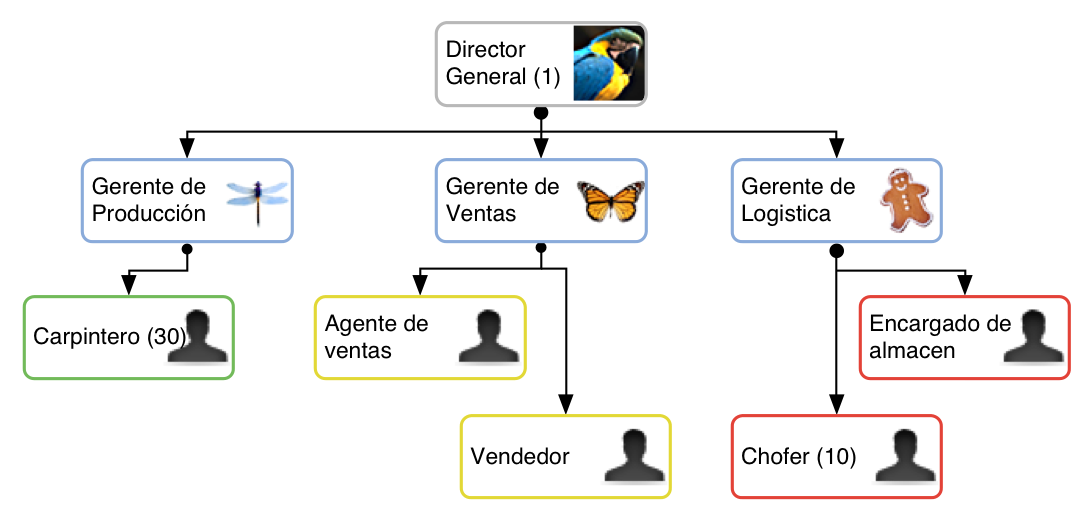
\includegraphics[width=.8\textwidth]{images/organigramaEm}
		\caption{Organigrama de la Mueblería Qetzal S. A. de C. V.}
		\label{fig:organigrama}
	\end{center}
\end{figure}


%---------------------------------------------------------
\section{Procesos involucrados}

\cdtInstrucciones{
	Coloque el mapa de procesos de la organización y liste a continuación los proceso que serán afectados por el desarrollo del sistema. Para cada proceso indique: Clave, Nombre y descripción.
}

\begin{figure}[htbp!]
	\begin{center}
		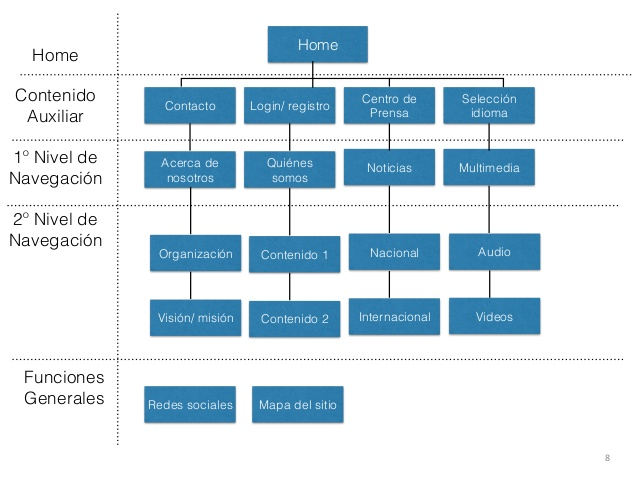
\includegraphics[width=.8\textwidth]{images/mapa}
		\caption{Mapa de procesos de la Mueblería Qetzal S. A. de C. V.}
		\label{fig:mapaProcASIS}
	\end{center}
\end{figure}

\begin{description}
	\item[PR-01] Nombre del proceso. Descripción del proceso.
\end{description}

%---------------------------------------------------------
\section{Requerimientos de usuario}

\cdtInstrucciones{
	Identifique y describa los requerimientos del usuario señalando: id, nombre, descripción y prioridad.
}

Los requerimientos del usuario son los siguientes\FootnoteStatus:

\begin{requerimientosU}
	\FRitem{RU-01}{Nombre del requerimiento}{Descripción del requerimiento.}{1}{\TODO}
	\FRitem{}{...}{...}{...}{...}
\end{requerimientosU}
\begin{table}[htbp]
\centering
\begin{tabular}{|c|l|p{10cm}|}
\hline
\textbf{ID} & \textbf{Nombre del Requerimiento} & \textbf{Descripción} \\ \hline
RNF1 & Seguridad básica de la Información & El sistema debe proteger los datos de los estudiantes y profesores mediante contraseñas y permisos de acceso por roles, implementando autenticación básica. \\ \hline
RNF2 & Disponibilidad del Sistema & El sistema debe estar disponible en horarios escolares y accesible de forma remota para los profesores y directores, con un tiempo de actividad mínimo del 90\%. \\ \hline
RNF3 & Tiempo de Respuesta & Las operaciones principales del sistema, como la consulta de información o actualización de datos, deben tener un tiempo de respuesta inferior a 3 segundos en entornos controlados de prueba. \\ \hline
RNF4 & Accesibilidad & El sistema debe cumplir con estándares de accesibilidad web (como WCAG 2.0), garantizando que los profesores y directores con discapacidades visuales o auditivas puedan usarlo sin dificultades. \\ \hline
RNF5 & Facilidad de mantenimiento & El sistema debe estar bien documentado para que otros estudiantes o profesores puedan mantenerlo y hacer mejoras sin dificultad. \\ \hline
RNF6 & Compatibilidad multiplataforma & El sistema debe ser accesible desde navegadores web comunes como Chrome o Firefox, y no requerir software adicional más allá de un navegador. \\ \hline
RNF7 & Interfaz amigable para usuarios & El sistema debe tener una interfaz sencilla y fácil de usar, con formularios claros y navegación intuitiva para profesores con poca experiencia técnica. \\ \hline
RNF8 & Copia de seguridad manual & El sistema debe permitir realizar copias de seguridad manuales de los datos educativos, exportando archivos en formatos como CSV o Excel para garantizar la conservación de la información. \\ \hline
RNF9 & Bajo costo de implementación & El sistema debe usar tecnologías y recursos gratuitos o de bajo costo para mantenerse dentro del presupuesto del proyecto. \\ \hline
RNF10 & Requerimientos técnicos mínimos & El sistema debe funcionar en computadoras con especificaciones mínimas (procesadores dual-core, 4GB de RAM, etc.), lo que lo hace viable para centros educativos con recursos limitados. \\ \hline
\end{tabular}
\caption{Requerimientos no funcionales para el sistema}
\end{table}
%---------------------------------------------------------
\section{Especificación de plataforma}	

\cdtInstrucciones{
	Coloque un diagrama y su descripción para aclarar el tipo de solución propuesta. \\
	
 En esta sección se debe aclarar:
	
\begin{description}
	\item[Tipo de sistema:] Web, aplicación móvil, de escritorio, híbrida, etc.
	\item[Software requerido:] Programas que se deberán instalar, desde el sistema operativo, compiladores, interpretes, servidores, etc.
	\item[Hardware requerido:] CPU, núcleos, velocidad, memoria, disco duro, etc.
	\item[servicios:] De conexión, seguridad, firewall, respaldo de energía, redundancia, uso de raids, etc.
\end{description}
}

\begin{figure}[htbp!]
	\begin{center}
		\fbox{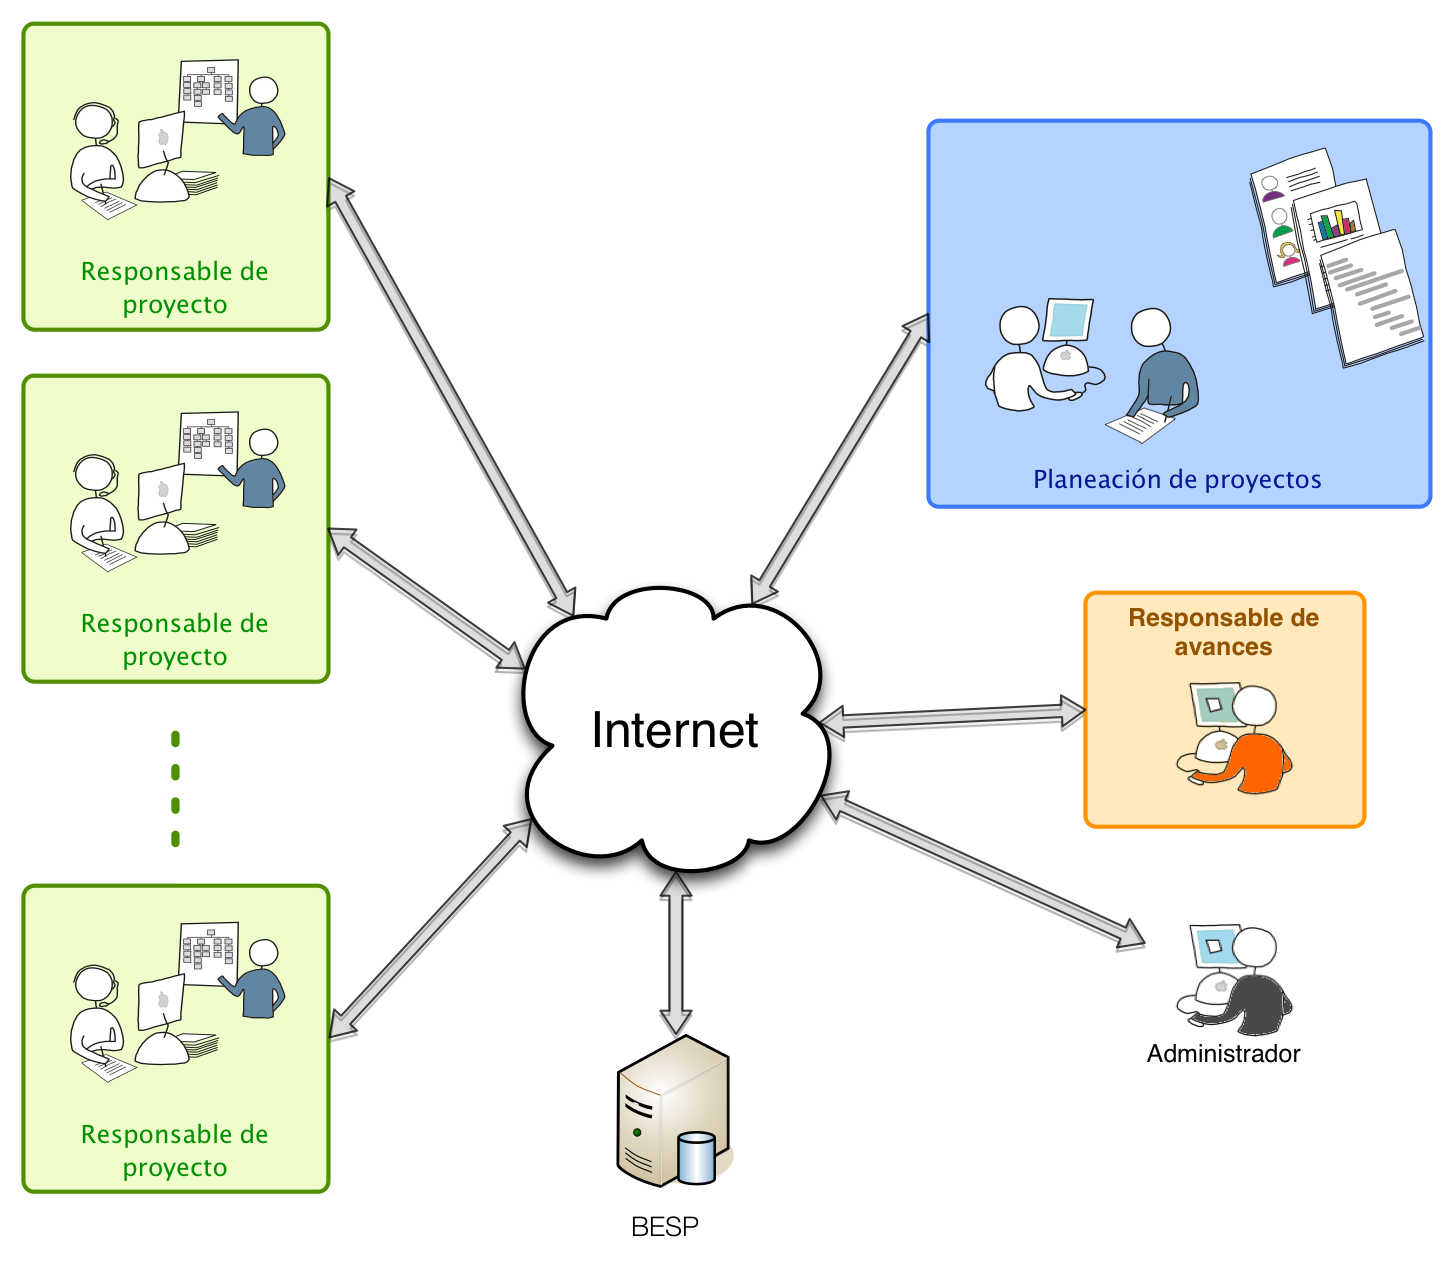
\includegraphics[width=.6\textwidth]{images/arquitectura}}
		\caption{Arquitectura del sistema.}
		\label{fig:arquitectura}
	\end{center}
\end{figure}

En la figura~\ref{fig:arquitectura} se describe la estructura del sistema, en ella se detalla ...




%=========================================================
% !TeX root = proyecto.tex

%=========================================================
\chapter{Modelo del Negocio}	
\label{cap:reqSist}

\cdtInstrucciones{Introduzca el capítulo describiendo el contenido del mismo, su organización y propósito.}

%----------------------------------------------------------
\section{Actores del sistema}

	\cdtInstrucciones{En esta sección describa a los actores del sistema.}
	
	%---------------------------------------------------------
	\begin{Usuario}{\hypertarget{A.NombreDelUsuario}{\subsection{Nombre del usuario}}}{
			Descripción del usuario: su puesto
		}
		\item[Responsabilidades:] \cdtEmpty
		\begin{itemize}
			\item Listar todas las responsabilidades y actividades dentro de la empresa.
			\item ...
		\end{itemize}
		
		\item[Perfil:] \cdtEmpty
		\begin{itemize}
			\item Describa el perfil del puesto: cursos, experiencia,habilidades blandas, escolaridad, certificaciones, etc.
			\item ...
		\end{itemize}
		\item[Procesos en los que participa:] \cdtEmpty
		\begin{itemize}
			\item Liste los procesos en los que participa.
			\item PC-V01 Aprobar las ordenes de compra al mayoreo.
			\item ...
		\end{itemize}
		\item[Área:] Indique el nombre del área a la que pertenece dentro de la organización
		\item[Cantidad aproximada:] Cantidad aproximada de personas que participan con este rol en el negocio.
		\item[Horario actividad:] En qué horario se espera que utilice el sistema. 
	\end{Usuario}
	
%---------------------------------------------------------
\section{Términos del Negocio}
\label{sec:terminosDeNegocio}

\cdtInstrucciones{En esta sección describa todos los términos del negocio que aparecen en la especificación del sistema.}
	
\begin{description}
	% Ejemplo de un término literal.
	\item[\hypertarget{tAutomovil}{Automóvil:}] ({\em es un tipo de \hyperlink{tVehiculo}{Vehículo}}) De cuatro ruedas con capacidad de 5 a 9 personas. 
	% Ejemplo de un término de entidad
	\item[\hypertarget{tCliente}{Cliente:}] Se refiere a todas las personas físicas y morales que \hyperlink{tRenta}{rentan} o han rentado un \hyperlink{tVehiculo}{vehículo}.
	
	\item[\hypertarget{tDirector}{Director:}] ({\em es un tipo de \hyperlink{tEmpleado}{Empleado}}) Es el empleado que tiene mayor rango de todos y no tiene superior, a diferencia de los demás.	
	\item[\hypertarget{tEmpleado}{Empleado:}] Se refiere a cualquier persona que labore en la empresa.
	
	\item[\hypertarget{tChecador}{Checador:}] ({\em Reloj asociado al atributo:} Hora de entrada y salida de un \hyperlink{tEmpleado}{empleado}. {\em Frecuencia de lectura:} Una vez al día para la entrada y otra para la salida durante los días laborales.
	
	\item[\hypertarget{tMotocicleta}{Motocicleta:}] ({\em es un tipo de {tVehiculo}{Vehículo}}) De dos ruedas con capacidad para una personas. 

	\item[\hypertarget{tRenta}{Renta:}] Se refiere al servicio que ofrece la empresa para prestar \hyperlink{tVehiculo}{vehículos} a los \hyperlink{tCliente}{clientes} por un tiempo definido.
	
	\item[\hypertarget{tVehiculo}{Vehiculo:}] Se refiere a los automóviles y motocicletas que la empresa usa para dar el servicio de renta a los \hyperlink{tCliente}{clientes}.
	
%	\brTermSensor{tVelocimetro}{Velocímetro:}{Velocidad de un Vehículo.}{Kilometros/hora.}{Constantemente siempre que el \cdtRef{tVehiculo}{vehículo} esté encendido.}
\end{description}

%----------------------------------------------------------
\section{Modelo del dominio del problema}
\label{sec:hechosDeNegocio}

\cdtInstrucciones{En esta sección describa todas las entidades del negocio y sus relaciones.}

	El modelo del dominio del problema se muestra en la figura~\ref{fig:modeloDeDominio}, a continuación se describen cada una de las entidades y sus relaciones.
	
\begin{figure}[htpb!]
	\begin{center}
		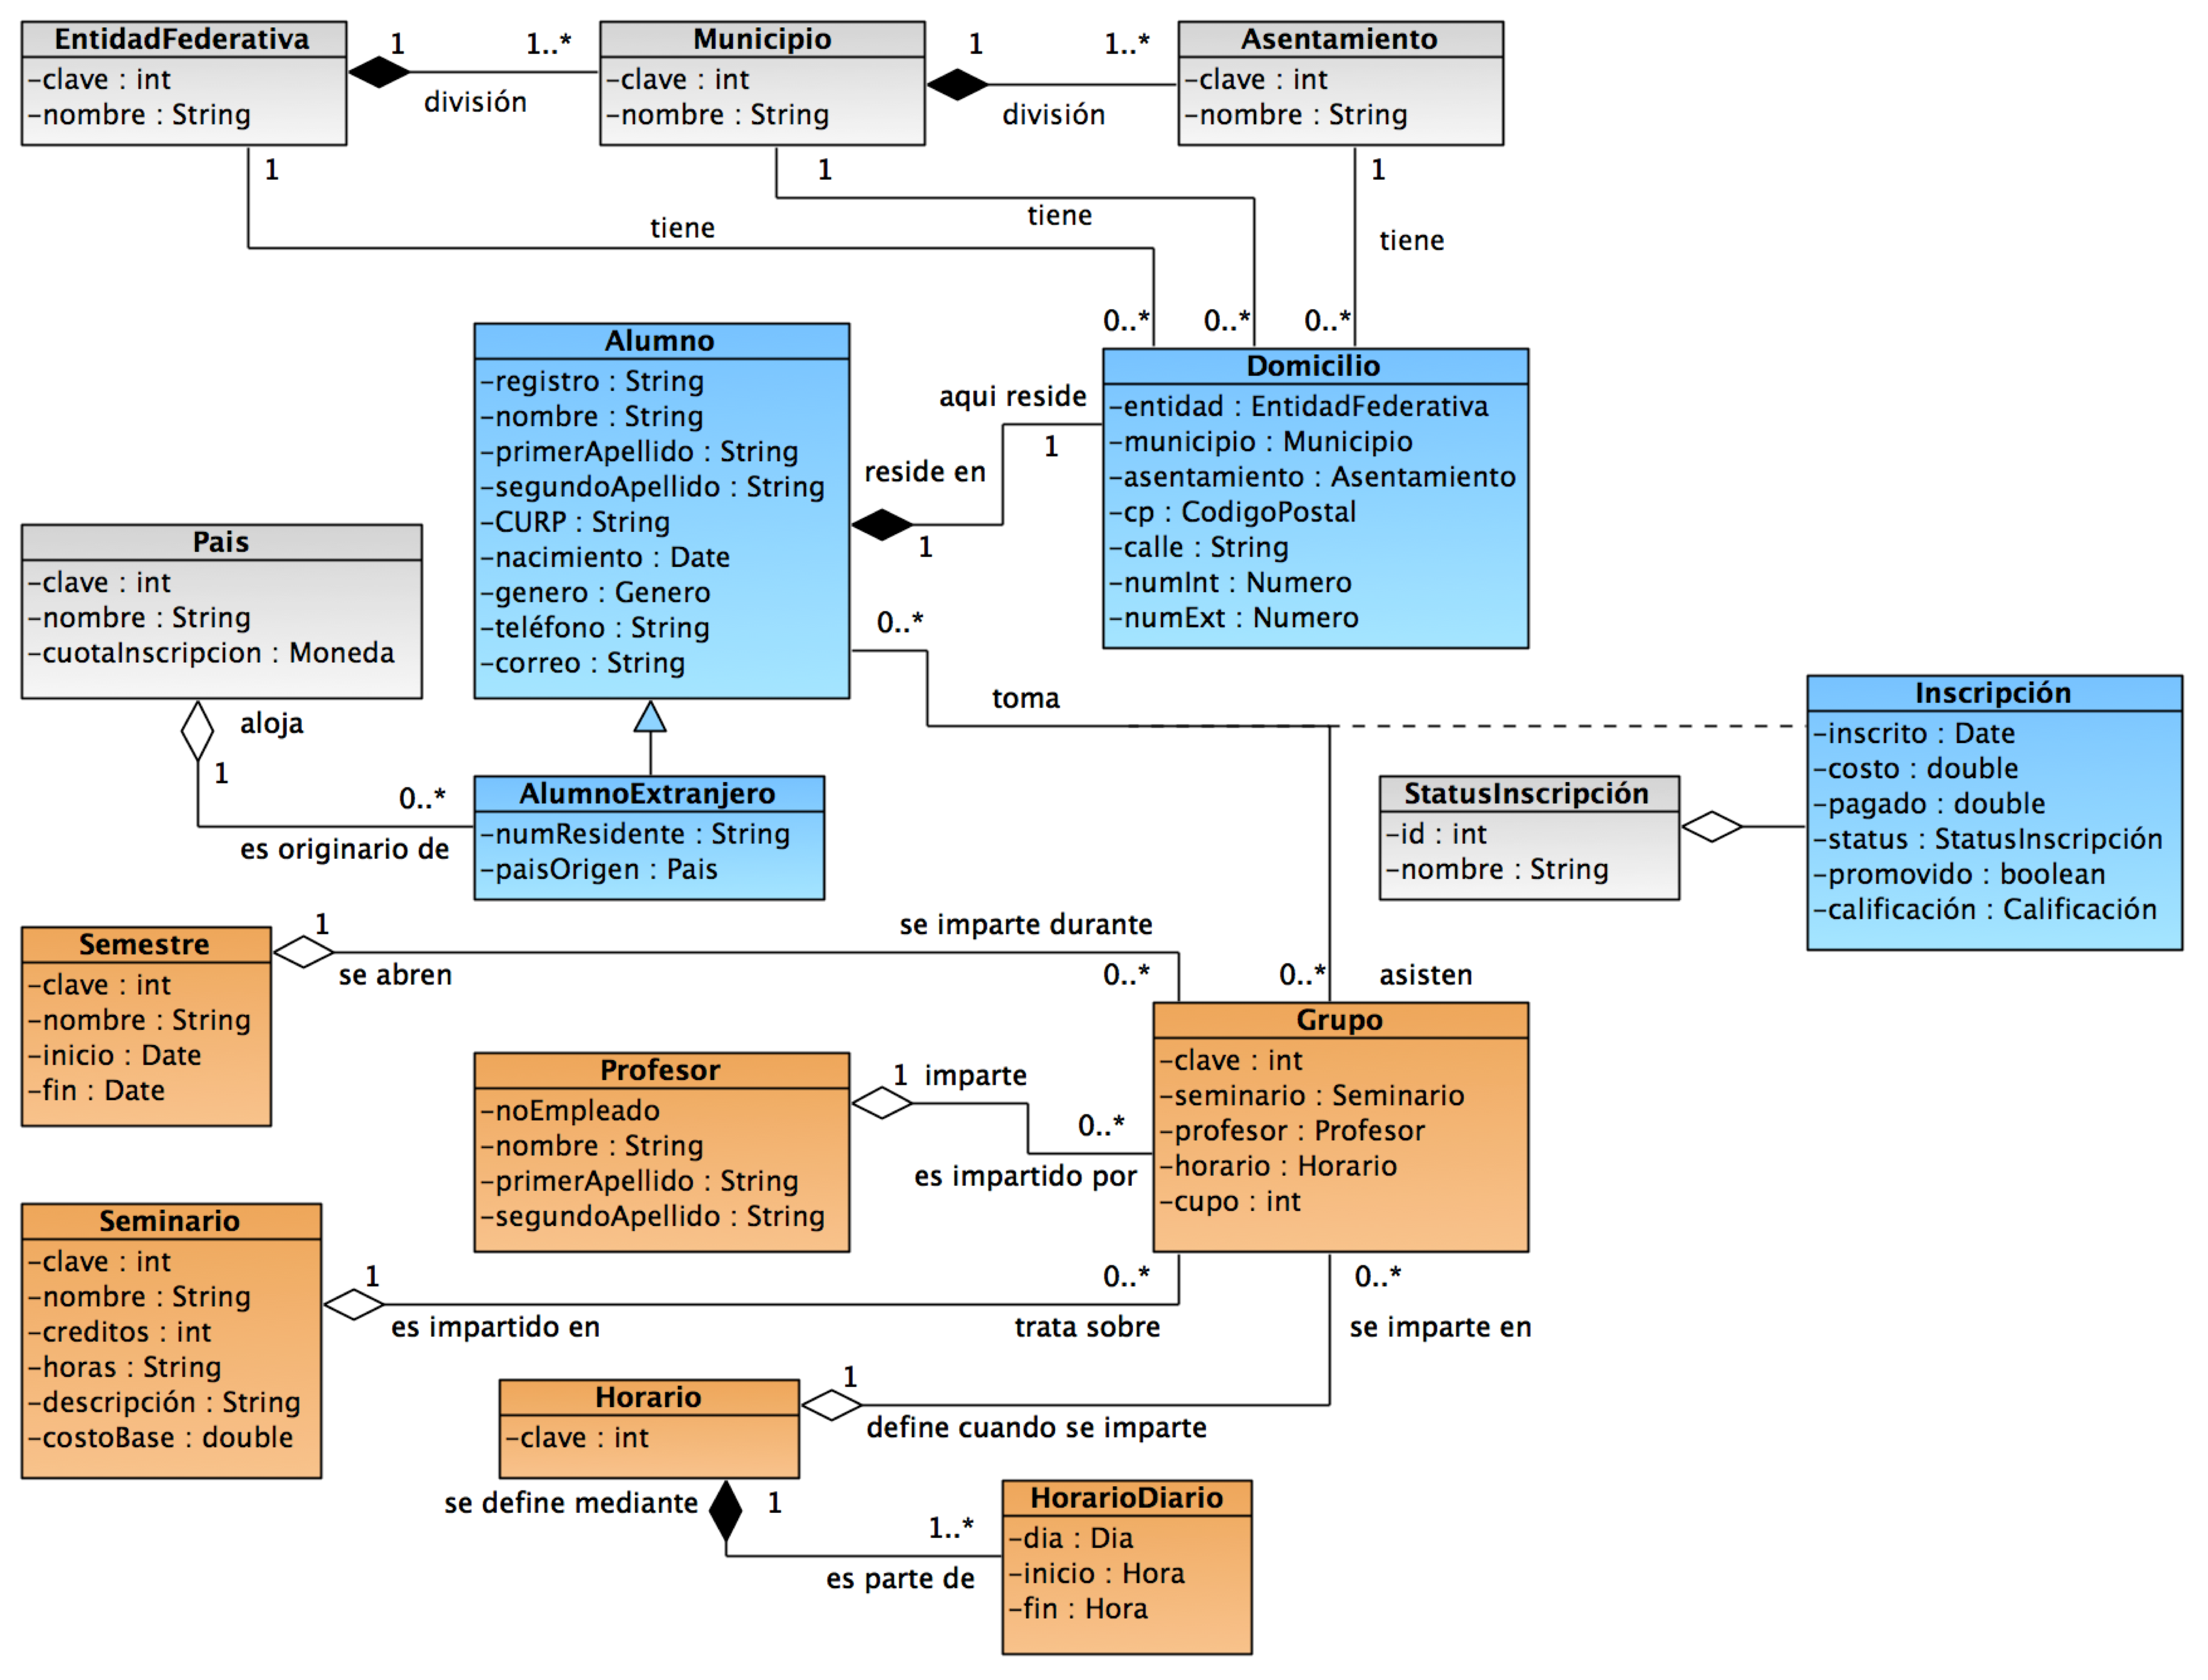
\includegraphics[angle=90,width=.95\textwidth]{images/modeloDelDominioDelProblema}
		\caption{Modelo del dominio del problema}
		\label{fig:modeloDeDominio}
	\end{center}
\end{figure}

\begin{cdtEntidad}{Alumno}{Alumno}
	\brAttr{registro}{Registro}{Id}{Número de registro utilizado para identificar un alumno}{Sí}
	\brAttr{nombre}{Nombre}{Palabra Corta}
		{Nombre o nombres del alumno.}{Sí}
	\brAttr{primerApellido}{Primer apellido}{Palabra Corta}
		{Primer apellido del alumno.}{Sí}
	\brAttr{segundoApellido}{Segundo apellido}{Palabra Corta}
		{Segundo apellido del alumno.}{No}
	\brAttr{CURP}{CURP}{CURP}
		{CURP del alumno.}{Sí}
	\brAttr{nacimiento}{Nacimiento}{Fecha}
		{Fecha de nacimiento del alumno.}{Sí}
	\brAttr{genero}{Género}{Domicilio}
		{Género del alumno.}{No}
	\brAttr{telefono}{Teléfono}{Telefono}
		{Teléfono para contactar al alumno.}{Sí}
	\brAttr{correo}{Correo}{Correo}
		{Correo del alumno para enviar información académica y escolar y para recuperación de clave de acceso.}{Sí}
	\cdtEntityRelSection
	\brRel{\brRelComposition}{Domicilio}{Un \hyperlink{Alumno}{Alumno} reside en un \hyperlink{Domicilio}{Domicilio}}	
	\brRel{\brRelAgregation}{Grupo}{Un \hyperlink{Alumno}{Alumno} toma un \hyperlink{Curso}{Curso}}	
\end{cdtEntidad}

%- - - - - - - - - - - - - - - - - - - - - - - - - - - - - 
\begin{cdtEntidad}{AlumnoExtranjero}{Alumno Extranjero}%{}
	\brAttr{numeroResidente}{Numero de residente}{Id}{Número de registro dado por la Secretaría de Relaciones Exteriores a los extranjeros.}{Si}
	\brAttr{paisOrigen}{Pais origen}{\hyperlink{Pais}{País}}
		{País de origen del alumno extranjero.}{Sí}
	\cdtEntityRelSection
	\brRel{\brRelAgregation}{País}{Un \hyperlink{Alumno}{Alumno} es originario de un \hyperlink{Pais}{Pais}}	
	\brRel{\brRelGeneralization}{Alumno}{Un \hyperlink{AlumnoExtranjero}{Alumno Extranjero} es un  \hyperlink{Alumno}{Alumno}}	
	\brRel{\brRelParticipation}{Alumno}{Un \hyperlink{AlumnoExtranjero}{Alumno Extranjero} es un  \hyperlink{Alumno}{Alumno}}	
\end{cdtEntidad}

%---------------------------------------------------------
\section{Modelado de Reglas de negocio}


% !TeX root = proyecto.tex


\cdtInstrucciones{En esta sección describa todas las reglas de negocio identificadas.}


% Tipo: \btDerivation (no aplica Clase), \btEnabler, \btTimer, \btExecutive
% Clase: \bcCondition, \bcIntegrity, \bcAutorization.
% Cumplimiento: \blStrict \blDeferred \blPreAutorized \blPostJustified \blOverride \blGuideline
\begin{BussinesRule}[%
	\brClassification{\btEnabler}{\bcCondition}{\blStrict}
	]{BR-001}{Nombre de la regla de negocio}
	
				% Opciones para nivel: \blControlling, \blInfluencing
	\BRitem[Descripción:] Descripción de la regla. Forma coloquial a manera de reglamento.
	\BRitem[Motivación:] Describa por que es importante la regla.
	\BRitem[Sentencia:] Sentencia formal de la regla.
	\BRitem[Ejemplo positivo:] Indique uno o varios ejemplos en donde la regla se cumple.
        \begin{itemize}
        	\item ...
        \end{itemize}
	
	\BRitem[Ejemplo negativo:] Indique uno o varios ejemplos en dónde la regla no se cumple.
		\begin{itemize}
        	\item ...
        \end{itemize}
	
	\BRitem[Referenciado por:] Liste los casos de uso en donde la regla no se cumple. por ejemplo \hyperlink{CUCE3.2}{CUCE3.2}, \hyperlink{CUCE3.3}{CUCE3.3}.
\end{BussinesRule}




\section{Máquinas de estado}

% !TeX root = proyecto.tex

\cdtInstrucciones{En esta sección describa para cada máquina de estados y a que entidad corresponde. Utilice reglas ECA en el diagrama y elabore el diagrama de estados, una descripción del diagrama, una descripción de cada estado y una descripción de las acciones indicando que casos de uso están involucrados.}

% - - - - - - - - - - - - - - - - - - - - - - - - - - - - 
\subsection{Estados para un préstamo}

En la figura~\ref{fig:edos-prestamo} se muestran ...

\begin{figure}[htbp]
	\begin{center}
		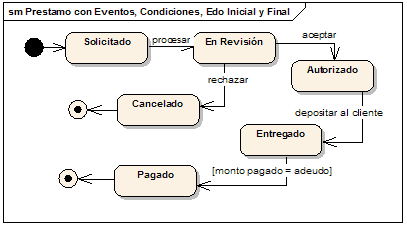
\includegraphics[width=.7\textwidth]{images/edoPrestamo}
		\caption{Máquina de estados de un Préstamo.}
		\label{fig:edos-prestamo}
	\end{center}
\end{figure}

\subsubsection{Estados}

\begin{description}
	\item[Estado:] Descripción del estado.
	\item[...] ...
\end{description}


\subsubsection{Acciones}

\begin{description}
	\item[Acción:] Descripción de la acción indicando el Caso de uso involucrado.
	\item[...] ...
\end{description}






%=========================================================
% !TeX root = proyecto.tex

%=========================================================
\chapter{Modelo dinámico}	
\label{cap:modDinamico}

\cdtInstrucciones{Presente la solución indicando el si esta se compone de varios sistemas, los subsistemas del sistema y si aplica, los módulos de los subsistemas.}

	Este capítulo describe en modelo dinámico del sistema. en el se detallan todos los escenarios de ejecución del sistema. La figura~\ref{fig:casosDeUso} muestra el diagrama general del sistema y sus subsistemas, y la figura~\ref{fig:casosDeUsoDetalle} muestra todos los casos de uso del sistema. En este documento solo detallamos los casos de uso del subsistema de gestión de cursos.
	
\begin{figure}[htbp]
	\begin{center}
		\fbox{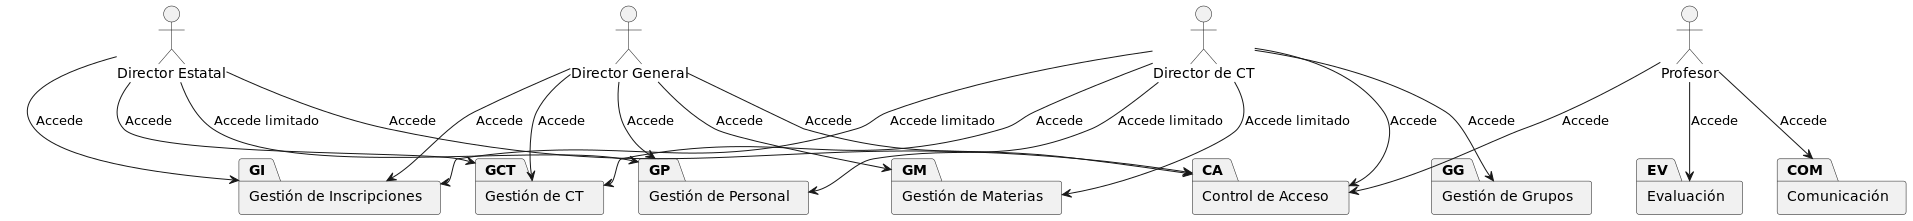
\includegraphics[width=.8\textwidth]{images/casosDeUso}}
		\caption{Diagrama de casos de uso del sistema.}
		\label{fig:casosDeUso}
	\end{center}
\end{figure}

\begin{figure}[htbp]
	\begin{center}
		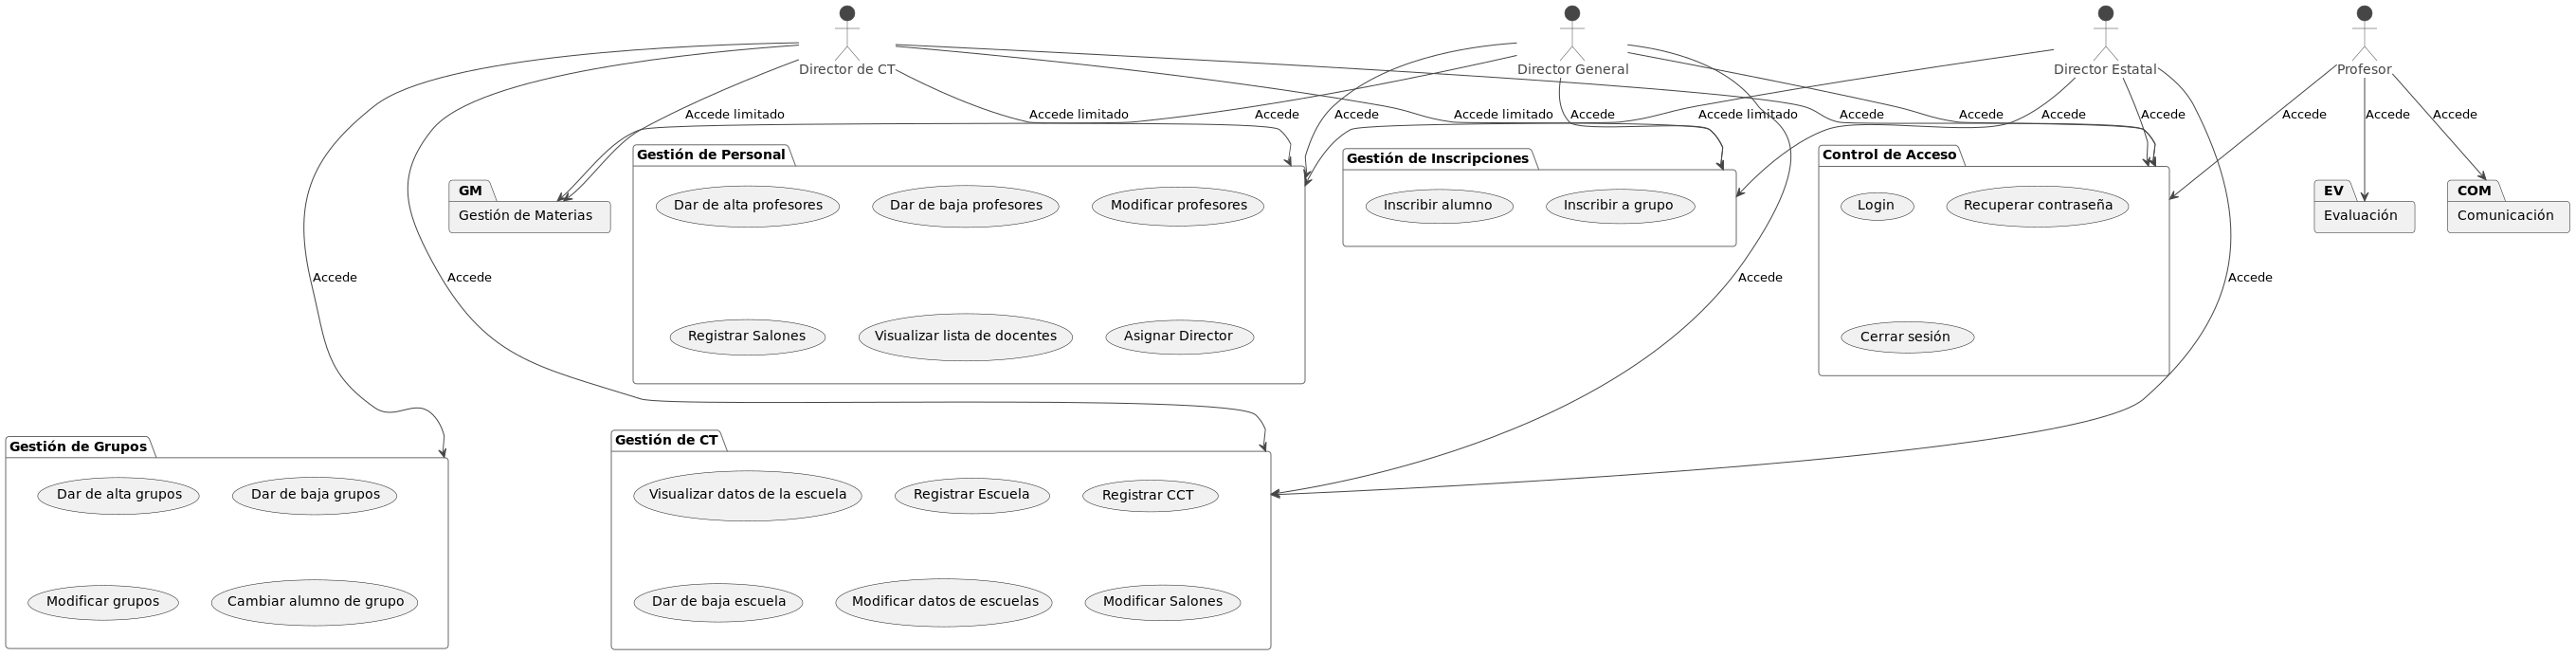
\includegraphics[ width=1.1\textwidth]{images/casosDeUsoDetalle}
		\caption{Diagrama detallado del sistema.}
		\label{fig:casosDeUsoDetalle}
	\end{center}
\end{figure}

%---------------------------------------------------------
\section{Descripción de casos de uso}



A continuación se detallan los casos de uso.

%---------------------------------------------------------
% CASOS DE USO

%%!TEX root = ../proyecto.tex

% Plantilla para caso de uso sencillo con ejemplos de comandos e intrucciones.
%-------------------------------------- COMIENZA descripción del caso de uso.

%\begin{UseCase}[archivo de imágen]{UCX}{Nombre del Caso de uso}{
%--------------------------------------
\begin{UseCase}{CUX}{Escriba el nombre del caso de uso}{
	% La descripción debe describir el evento de inicio del caso de uso, Breve descripción de la trayectoria y estado final del caso de uso.
}
	\UCitem{Versión}{\color{Gray}
		0.1	% Ponga un número de versión, 
	}\UCitem{Autor}{\color{Gray}
		Nombre del analista. % Analista responsable de especificar el CU
	}\UCitem{Supervisa}{\color{Gray}
		Nombre del analista revisor. % Analista responsable de verificar que está correcto.
	% TODO: Dar de alta al actor Usuario
	}\UCitem{Actor}{
		\hyperlink{IdDelActor}{Nombre del actor} % No olvide dar de alta el actor.
	}\UCitem{Propósito}{\begin{Titemize}%Indique los fines, objetivos, propósitos o valores agregados del Caso de uso.
		\Titem Propósito del caso de uso.
		\Titem ...
	\end{Titemize}
	}\UCitem{Entradas}{\begin{Titemize}
		% TODO: Dar de alta las entidades que se listan.
		\Titem \hyperlink{Entidad.Atributo}{Nombre del dato de entrada}. % El identificador no acepta acentos, espacios ni eñes.
		\Titem \hyperlink{Entidad.Atributo}{Nombre del dato de entrada}. % Liste todos los datos de entrada
		\end{Titemize}
	}\UCitem{Origen}{\begin{Titemize}
		\Titem Se introducen desde el teclado. % Indique por que medio se introducen los datos, 
		\Titem otros.          % Si es ḿas de uno indique que datos corresponden en cada medio de entrada.
	\end{Titemize}
	}\UCitem{Salidas}{\begin{Titemize}
		% TODO: Dar de alta las entidades que se listan.
		\Titem \hyperlink{Entidad.Atributo}{Nombre del dato de entrada}.
		\Titem Mensajes de error. % Indique por que medio se introducen los datos, 
		\Titem Datos que aparecen en pantalla.          % Si es ḿas de uno indique que datos corresponden en cada medio de entrada.
		\Titem Datos que aparecen en listas desplegables o tablas, etc.
		\Titem Datos que se imprimen o que se envía a otros sistemas.
	\end{Titemize}
	}\UCitem{Destino}{\begin{Titemize}
		\Titem Se muestra en la pantalla \IUref{IUX}{Nombre pantalla}.. % Indique por que medio se muestran los datos, 
		\Titem otros.          % Si es ḿas de uno indique que datos corresponden en cada medio de entrada.
	\end{Titemize}
	}\UCitem{Precondiciones}{\begin{Titemize}
		% Incluya Precondiciones lógicas, de negocio e incluso las que debe atender el usuario. 
		% Muchas precondiciones provienen de reglas de negocios, otras estarán asociadas a manejo de errores
		% Otras están relacionadas con casos de uso que deben ejecutarse previamente, como registrar un producto.
		\Titem Escriba la precondición.
	\end{Titemize}
	}\UCitem{Postcondiciones}{\begin{Titemize}
		% Indique todas las postcondiciones
		% por ejemplo, Cambios en el sistema
		% Cambios en la BD una vez terminado el CU
		% Efectos colaterales
		% Condiciones de término.
		\Titem Escriba todas las postcondiciones.
	\end{Titemize}
	}\UCitem{Errores}{\begin{Titemize}
		% Escriba todos los errores que puedan ocurrir en el sistema, para cada error recuerde:
		% Punerle un identificador
		% Describir la condición o escenario que detona el error
		% Describa la forma en que debe reaccionar el sitema: si la reaccion corresponde a varios pasos use mejor una trayectoria alternativa.
		% Relacione el error con la trayectoria principal.
		\Titem {\bf \hypertarget{CUX.E1}{E1}}: Condición que detona el error, reacción del sistema y regresa al paso \ref{UC1.etiqueta}.
		\Titem {\bf \hypertarget{CUX.E2}{E2}}: Condición que detona el error, reacción del sistema y termina el Caso de uso..
	\end{Titemize}
	}\UCitem{Tipo}{
		% Especifique el tipo de caso de us, puede ser: "Caso de uso primario" o 
		% "Viene de \\hyperref{CUY}{CUY nombre del CU}" cuando se desprende desde otro caso de uso mediante un extends.
		Caso de uso primario
	}\UCitem{Observaciones}{
		% Indique las observaciones al caso de uso, las cuales pueden ser:
		% - Ninguna
		% - Dudas sobre el procedimiento o la especificación.
		% - Issues detectados
		% - Suposiciones realizadas.
		% - Cualquier otra especificacion que considere pertinente que no pudo colocarse en los demás atributos del Caso de uso
		% - Aclaraciones.
		% - Notas para el usuario o desarrollador.
		% - Pendientes (TODO's) en caso de no usar los comentarios.
	}
\end{UseCase}

%--------------------------------------
\begin{UCtrayectoria}
	% Cada paso debe inicair con un Verbo en infinitivo, siempre especificando el objetivo del paso mas la accion en concreto.
	% \UCpaso[\UCactor] se refiere al actor y \UCpaso se refiere al sistema.
	% A continuación viene ejemplos de pasos:
	% En el siguiente paso: "Ingresa al sistema" es el objetivo del paso y "escribiendo la URL de la aplicación" es la acción en concreto.
	\UCpaso[\UCactor o \UCsist] VERBO EN INFINITIVO + (Acción del usuario) + (Acción dentro del sistema)
	\UCpaso[\UCactor] Ingresa al sistema escribiendo la URL de la aplicación.
	% En el siguinte paso se referencia una Interfaz:
	\UCpaso Solicita al usuario que se identifique mediante la pantalla \IUref{IU1}{Inicio de sesión}
	% En el siguiente paso está etiquetado para ser referenciado por un error o trayectoria alternativa:
	\UCpaso[\UCactor] \label{UCX.introduceDatos} Se identifica introduciendo su nombre de usuario y contraseña.
	% En el siguiente paso se usa el comando \IUbutton 
	\UCpaso[\UCactor] Solicita el ingreso al sistema presiona el botón \IUbutton{Ingresar}.
	% En el siguiente paso se referencía un error.
	\UCpaso Busca los datos del usuario identificado por el nombre de usuario introducido \ErrorRef{CUX}{E1}{No hay usuario}
	% En el siguiente paso se señala una trayectoria alternativa
	\UCpaso Verifica que el usuario especificado no esté inactivo \ErrorRef{CUX}{E2}{Usuario inactivo} \Trayref{CUX}{A}.
	% En el siguiente paso se referencían dos errores y una trayectoria alternativa.
	\UCpaso Verifica que la contraseña ingresada coincida con la almacenada \ErrorRef{CUX}{E3}{La contraseña no coincide}\Trayref{CUX}{B}.
	% En el siguiente paso se señala la incusión de otro CU
	\UCpaso[] Se ejecutan los pasos del caso de uso \UCref{CUY}{Nombre del caso de uso}.
	% En el siguiente paso se señala un mensaje.
	\UCpaso Muestra la pantalla \IUref{IU2}{Principal} con el mensaje \MSGref{MSG-001}{Bienvenida al usuario}.
\end{UCtrayectoria}


%--------------------------------------
% Las trayectorias alternativas se identifican con Letras: A, B, C, etc.
\begin{UCtrayectoriaA}{CUX}{LETRA}{Condición que hace que se ejecute esta trayectoria}
	\UCpaso Especifique los pasos  de la trayectoria.
	% Se puede desprender otra trayectria alternativa si es necesario.
	% Finalice la trayectoria indicando si la ejecución se integra a la trayectoria anterior o si termina la ejecución del CU.
	% Verifique que la redacción de la trayectoria deje en claro si el objetivo del CU se alcanzó o no.
	\UCpaso[] El Caso de Uso continúa en el paso \ref{UCX.introduceDatos}.
\end{UCtrayectoriaA}


%--------------------------------------
% Puntos de extensión

% Comente la siguiente sección en caso de que no hayan puntos de extensión o relaciones de tipo extends.
\subsection{Puntos de extensión}
\UCExtenssionPoint{
	% Cuando se dá la extensión del Caso de uso:
	El usuario no recuerda cual es su contraseña o sospecha que su usuario está bloqueado.
}{
	% Durante la región (en que pasos se puede dar la extensión):
	Del paso \ref{CUX.etiqueta} al paso \ref{CUX.etiqueta}.
}{
	% Casos de uso a los que extiende:
	\UCref{CUZ}{Nombre del caso de uso}.
}
		
		
		
%-------------------------------------- TERMINA descripción del caso de uso.
%!TEX root = ../proyecto.tex

% Plantilla para caso de uso sencillo con ejemplos de comandos e intrucciones.
%-------------------------------------- COMIENZA descripción del caso de uso.

%\begin{UseCase}[archivo de imágen]{UCX}{Nombre del Caso de uso}{
%--------------------------------------
\begin{UseCase}{CU-001}{Inicio de sesión (login) }{
	% La descripción debe describir el evento de inicio del caso de uso, Breve descripción de la trayectoria y estado final del caso de uso.
 Cuando un usuario desee ingresar al sistema deberá proporcionarle sus datos de acceso y de ser correctos este le permitirá iniciar sesión.
}
	\UCitem{Versión}{\color{Gray}
		0.1	% Ponga un número de versión, 
	}\UCitem{Autor}{\color{Gray}
		Agustín Flores López. % Analista responsable de especificar el CU
	}\UCitem{Supervisa}{\color{Gray}
		Juan Ángel Serrano Carreño . % Analista responsable de verificar que está correcto.
	% TODO: Dar de alta al actor Usuario
	}\UCitem{Actor}{
		\hyperlink{Usuarios}{Usuarios} % No olvide dar de alta el actor.
	}\UCitem{Propósito}{\begin{Titemize}%Indique los fines, objetivos, propósitos o valores agregados del Caso de uso.
		\Titem Controlar el acceso al sistema.
		\Titem Restringir el uso de las funciones más sensibles solo a los perfiles adecuados.
        \Titem Permitir la trazabilidad de las operaciones en el sistema.
	\end{Titemize}
	}\UCitem{Entradas}{\begin{Titemize}
		% TODO: Dar de alta las entidades que se listan.
		\Titem \hyperlink{Usuario.ID}{Identificador} en el PRONIM. % El identificador no acepta acentos, espacios ni eñes.
		\Titem \hyperlink{Usuario.Contrasenia}{Contraseña}. % Liste todos los datos de entrada
		\end{Titemize}
	}\UCitem{Origen}{\begin{Titemize}
		\Titem Se introducen desde el teclado. % Indique por que medio se introducen los datos,           % Si es ḿas de uno indique que datos corresponden en cada medio de entrada.
	\end{Titemize}
	}\UCitem{Salidas}{\begin{Titemize}
		% TODO: Dar de alta las entidades que se listan.
		\Titem \hyperlink{Usuario.nombre}{Nombre} del \hyperlink{Usuario}{Usuario}.
            \Titem \hyperlink{Usuario.primerApellido}{Primer apellido} del \hyperlink{Usuario}{Usuario}.
		\Titem Mensajes de error. % Indique por que medio se introducen los datos, 
		         % Si es ḿas de uno indique que datos corresponden en cada medio de entrada.
		
	\end{Titemize}
	}\UCitem{Destino}{\begin{Titemize}
		\Titem Se muestra en la pantalla \IUref{IU001}{Inicio de sesión}.. % Indique por que medio se muestran los datos, 
          % Si es ḿas de uno indique que datos corresponden en cada medio de entrada.
	\end{Titemize}
	}\UCitem{Precondiciones}{\begin{Titemize}
		% Incluya Precondiciones lógicas, de negocio e incluso las que debe atender el usuario. 
		% Muchas precondiciones provienen de reglas de negocios, otras estarán asociadas a manejo de errores
		% Otras están relacionadas con casos de uso que deben ejecutarse previamente, como registrar un producto.
		\Titem El usuario debe estar registrado en el sistema.
	\end{Titemize}
	}\UCitem{Postcondiciones}{\begin{Titemize}
		% Indique todas las postcondiciones
		% por ejemplo, Cambios en el sistema
		% Cambios en la BD una vez terminado el CU
		% Efectos colaterales
		% Condiciones de término.
		\Titem El usuario inicia sesión en el sistema.
            \Titem El usuario puede acceder a las funciones de su rol.
	\end{Titemize}
	}\UCitem{Errores}{\begin{Titemize}
		% Escriba todos los errores que puedan ocurrir en el sistema, para cada error recuerde:
		% Punerle un identificador
		% Describir la condición o escenario que detona el error
		% Describa la forma en que debe reaccionar el sitema: si la reaccion corresponde a varios pasos use mejor una trayectoria alternativa.
		% Relacione el error con la trayectoria principal.
		\Titem {\bf \hypertarget{CU001.E1}{E1}}: Si el usuario olvida ingresar alguno de los campos obligatorios, el sistema mostrara el \MSGref{MSG-005}{Faltan rellenar campos obligatorios}. y regresa al paso \ref{UC1.Datos}.
		\Titem {\bf \hypertarget{CU001.E2}{E2}}: Si la contraseña es incorrecta, el sistema mostrara el \MSGref{MSG-004}{Error al iniciar sesión}  y regresa al paso \ref{UC1.Datos}.
  \Titem {\bf \hypertarget{CU001.E3}{E3}}: Si la cuenta esta inactiva, el sistema mostrara el \MSGref{MSG-003}{Cuenta inactiva}  y regresa al paso \ref{UC1.Datos}.
  \Titem {\bf \hypertarget{CU001.E4}{E4}}: Si la cuenta no existe, el sistema mostrara el \MSGref{MSG-002}{Usuario no registrado}  y regresa al paso \ref{UC1.Datos}.
	\end{Titemize}
	}\UCitem{Tipo}{
		% Especifique el tipo de caso de us, puede ser: "Caso de uso primario" o 
		% "Viene de \\hyperref{CUY}{CUY nombre del CU}" cuando se desprende desde otro caso de uso mediante un extends.
		Caso de uso primario
	}\UCitem{Observaciones}{
		% Indique las observaciones al caso de uso, las cuales pueden ser:
		% - Ninguna
		% - Dudas sobre el procedimiento o la especificación.
		% - Issues detectados
		% - Suposiciones realizadas.
		% - Cualquier otra especificacion que considere pertinente que no pudo colocarse en los demás atributos del Caso de uso
		% - Aclaraciones.
		% - Notas para el usuario o desarrollador.
		% - Pendientes (TODO's) en caso de no usar los comentarios.
	}
\end{UseCase}

%--------------------------------------
\begin{UCtrayectoria}
	% Cada paso debe inicair con un Verbo en infinitivo, siempre especificando el objetivo del paso mas la accion en concreto.
	% \UCpaso[\UCactor] se refiere al actor y \UCpaso se refiere al sistema.
	% A continuación viene ejemplos de pasos:
	% En el siguiente paso: "Ingresa al sistema" es el objetivo del paso y "escribiendo la URL de la aplicación" es la acción en concreto.
	
	\UCpaso[\UCactor] Ingresa al sistema escribiendo la URL de la aplicación.
	% En el siguinte paso se referencia una Interfaz:
	\UCpaso Solicita al usuario que se identifique mediante la pantalla \IUref{IU1}{Inicio de sesión}
	% En el siguiente paso está etiquetado para ser referenciado por un error o trayectoria alternativa:
	\UCpaso[\UCactor] \label{UC1.Datos} Se identifica introduciendo su Identificador de Pronim y contraseña.
	% En el siguiente paso se usa el comando \IUbutton 
	\UCpaso[\UCactor] Solicita el ingreso al sistema presiona el botón \IUbutton{Ingresar}.
	% En el siguiente paso se referencía un error.
    \UCpaso Verifica que todos los campos obligatorios esten llenos \ErrorRef{CU001}{E1}{Campos faltantes}.
	\UCpaso Busca los datos del usuario identificado por el Identificador introducido \ErrorRef{CU001}{E4}{Usuario no registrado}
	% En el siguiente paso se señala una trayectoria alternativa
	\UCpaso Verifica que el usuario especificado no esté inactivo \ErrorRef{CU001}{E3}{Usuario inactivo}.
	% En el siguiente paso se referencían dos errores y una trayectoria alternativa.
	\UCpaso Verifica que la contraseña ingresada coincida con la almacenada \ErrorRef{CU001}{E2}{La contraseña no coincide}.\label{UC1.Contrasenia}
	% En el siguiente paso se señala la incusión de otro CU
	\UCpaso Verifica su rol dentro del sistema y le otorga los permisos correspondientes
	% En el siguiente paso se señala un mensaje.
	\UCpaso Muestra la pantalla \IUref{IU2}{Principal} con el mensaje \MSGref{MSG-001}{Bienvenida al usuario}.
\end{UCtrayectoria}


%--------------------------------------
% Las trayectorias alternativas se identifican con Letras: A, B, C, etc.



%--------------------------------------
% Puntos de extensión

% Comente la siguiente sección en caso de que no hayan puntos de extensión o relaciones de tipo extends.
\subsection{Puntos de extensión}
\UCExtenssionPoint{
	% Cuando se dá la extensión del Caso de uso:
	El usuario no recuerda cual es su contraseña .
}{
	% Durante la región (en que pasos se puede dar la extensión):
	Del paso \ref{UC1.Datos} al paso \ref{UC1.Contrasenia}.
}{
	% Casos de uso a los que extiende:
	\UCref{CUX}{Nombre del caso de uso}.
}
		
		
		
%-------------------------------------- TERMINA descripción del caso de uso.
%!TEX root = ../proyecto.tex

% Plantilla para caso de uso sencillo con ejemplos de comandos e intrucciones.
%-------------------------------------- COMIENZA descripción del caso de uso.

%\begin{UseCase}[archivo de imágen]{UCX}{Nombre del Caso de uso}{
%--------------------------------------
\begin{UseCase}{CU-002}{Visualizar lista de escuelas (Suponiendo filtro y sesión necesaria)}{
	% La descripción debe describir el evento de inicio del caso de uso, Breve descripción de la trayectoria y estado final del caso de uso.
 Dado un inicio de sesión exitoso, el usuario puede dar clic en consultar escuelas,lo cual lo llevara a la IU002 que cambiara su contenido dependiendo del filtro aplicado por el usuario (Nombre de escuela,Nivel educativo,Estado,Lenguas)
}
	\UCitem{Versión}{\color{Gray}
		0.1	% Ponga un número de versión, 
	}\UCitem{Autor}{\color{Gray}
		Juan Ángel Serrano Carreño. % Analista responsable de especificar el CU
	}\UCitem{Supervisa}{\color{Gray}
		Agustín Flores López. % Analista responsable de verificar que está correcto.
	% TODO: Dar de alta al actor Usuario
	}\UCitem{Actor}{
		\hyperlink{Usuarios}{Usuarios} % No olvide dar de alta el actor.
	}\UCitem{Propósito}{\begin{Titemize}%Indique los fines, objetivos, propósitos o valores agregados del Caso de uso.
		\Titem Consultar la disponibilidad del PRONIM en una zona especifica
        \Titem Filtrar las escuelas que cumplan alguna de las siguientes características (Nombre de escuela,Nivel educativo,Estado,Lenguas)
	\end{Titemize}
	}\UCitem{Entradas}{\begin{Titemize}
		% TODO: Dar de alta las entidades que se listan.
        \Titem Nombre de la escuela (opcional)
		\Titem Nombre del estado (opcional)
        \Titem Escolaridad (opcional)
        \Titem Lenguas que permite (opcional)
		\end{Titemize}
	}\UCitem{Origen}{\begin{Titemize}
		\Titem Se introducen desde el teclado y el mouse para los selectores. % Indique por que medio se introducen los datos,           % Si es ḿas de uno indique que datos corresponden en cada medio de entrada.
	\end{Titemize}
	}\UCitem{Salidas}{\begin{Titemize}
		% TODO: Dar de alta las entidades que se listan.
		\Titem Listado de escuelas que cumplan con los filtros y que al dar clic los lleve al perfil de la escuela
        \Titem Mensaje de información 
	\end{Titemize}
	}\UCitem{Destino}{\begin{Titemize}
		\Titem Se muestra en la pantalla \IUref{IU002}{Listas de escuelas}.. % Indique por que medio se muestran los datos, 
          % Si es ḿas de uno indique que datos corresponden en cada medio de entrada.
	\end{Titemize}

% AQUI ME QUEDE
 
	}\UCitem{Precondiciones}{\begin{Titemize}
		% Incluya Precondiciones lógicas, de negocio e incluso las que debe atender el usuario. 
		% Muchas precondiciones provienen de reglas de negocios, otras estarán asociadas a manejo de errores
		% Otras están relacionadas con casos de uso que deben ejecutarse previamente, como registrar un producto.
		\Titem Debe haber un login exitoso en la plataforma.
	\end{Titemize}
	}\UCitem{Postcondiciones}{\begin{Titemize}
		% Indique todas las postcondiciones
		% por ejemplo, Cambios en el sistema
		% Cambios en la BD una vez terminado el CU
		% Efectos colaterales
		% Condiciones de término.
		\Titem Modificación de la lista a mostrar.
	\end{Titemize}
	}\UCitem{Errores}{\begin{Titemize}
		% Escriba todos los errores que puedan ocurrir en el sistema, para cada error recuerde:
		% Punerle un identificador
		% Describir la condición o escenario que detona el error
		% Describa la forma en que debe reaccionar el sitema: si la reaccion corresponde a varios pasos use mejor una trayectoria alternativa.
		% Relacione el error con la trayectoria principal.
		\Titem {\bf \hypertarget{CU002.E1}{E1}}: Dado una selección de filtros, no se encontró ningún elemento que los cumpla de forma que mostrara \MSGref{MSG-006}{No se encontró información}.
	\end{Titemize}
	}\UCitem{Tipo}{
		% Especifique el tipo de caso de us, puede ser: "Caso de uso primario" o 
		% "Viene de \\hyperref{CUY}{CUY nombre del CU}" cuando se desprende desde otro caso de uso mediante un extends.
		Caso de uso primario
	}\UCitem{Observaciones}{
		% Indique las observaciones al caso de uso, las cuales pueden ser:
		% - Ninguna
		% - Dudas sobre el procedimiento o la especificación.
		% - Issues detectados
		% - Suposiciones realizadas.
		% - Cualquier otra especificacion que considere pertinente que no pudo colocarse en los demás atributos del Caso de uso
		% - Aclaraciones.
		% - Notas para el usuario o desarrollador.
		% - Pendientes (TODO's) en caso de no usar los comentarios.
        Tiene que incluir los filtros y que se pueda ver unicamente si esta iniciado en sesión 
	}
\end{UseCase}

%--------------------------------------
\begin{UCtrayectoria}
	% Cada paso debe inicair con un Verbo en infinitivo, siempre especificando el objetivo del paso mas la accion en concreto.
	% \UCpaso[\UCactor] se refiere al actor y \UCpaso se refiere al sistema.
	% A continuación viene ejemplos de pasos:
	% En el siguiente paso: "Ingresa al sistema" es el objetivo del paso y "escribiendo la URL de la aplicación" es la acción en concreto.
	\UCpaso[\UCactor] Ingresa a la búsqueda de escuela dando clic en la opción buscar escuela de la interfaz principal (pendiente)
	% En el siguinte paso se referencia una Interfaz:
	\UCpaso Solicita al usuario que se identifique mediante la pantalla \IUref{IU2}{Listar escuelas}
	% En el siguiente paso está etiquetado para ser referenciado por un error o trayectoria alternativa:
	\UCpaso[\UCactor] \label{UCX.introduceDatos} Se identifica introduciendo su nombre de usuario y contraseña.
	% En el siguiente paso se usa el comando \IUbutton 
	\UCpaso[\UCactor] Solicita el ingreso al sistema presiona el botón \IUbutton{Ingresar}.
	% En el siguiente paso se referencía un error.
	\UCpaso Busca los datos del usuario identificado por el nombre de usuario introducido \ErrorRef{CUX}{E1}{No hay usuario}
	% En el siguiente paso se señala una trayectoria alternativa
	\UCpaso Verifica que el usuario especificado no esté inactivo \ErrorRef{CUX}{E2}{Usuario inactivo} \Trayref{CUX}{A}.
	% En el siguiente paso se referencían dos errores y una trayectoria alternativa.
	\UCpaso Verifica que la contraseña ingresada coincida con la almacenada \ErrorRef{CUX}{E3}{La contraseña no coincide}\Trayref{CUX}{B}.
	% En el siguiente paso se señala la incusión de otro CU
	\UCpaso[] Se ejecutan los pasos del caso de uso \UCref{CUY}{Nombre del caso de uso}.
	% En el siguiente paso se señala un mensaje.
	\UCpaso Muestra la pantalla \IUref{IU2}{Principal} con el mensaje \MSGref{MSG-001}{Bienvenida al usuario}.
\end{UCtrayectoria}


%--------------------------------------
% Las trayectorias alternativas se identifican con Letras: A, B, C, etc.
\begin{UCtrayectoriaA}{CUX}{LETRA}{Condición que hace que se ejecute esta trayectoria}
	\UCpaso Especifique los pasos  de la trayectoria.
	% Se puede desprender otra trayectria alternativa si es necesario.
	% Finalice la trayectoria indicando si la ejecución se integra a la trayectoria anterior o si termina la ejecución del CU.
	% Verifique que la redacción de la trayectoria deje en claro si el objetivo del CU se alcanzó o no.
	\UCpaso[] El Caso de Uso continúa en el paso \ref{UCX.introduceDatos}.
\end{UCtrayectoriaA}


%--------------------------------------
% Puntos de extensión

% Comente la siguiente sección en caso de que no hayan puntos de extensión o relaciones de tipo extends.
\subsection{Puntos de extensión}
\UCExtenssionPoint{
	% Cuando se dá la extensión del Caso de uso:
	El usuario no recuerda cual es su contraseña o sospecha que su usuario está bloqueado.
}{
	% Durante la región (en que pasos se puede dar la extensión):
	Del paso %\ref{CUX.etiqueta} al paso \ref{CUX.etiqueta}.
}{
	% Casos de uso a los que extiende:
	\UCref{CUZ}{Nombre del caso de uso}.
}
		
		
		
%-------------------------------------- TERMINA descripción del caso de uso.
%!TEX root = ../proyecto.tex

% Plantilla para caso de uso sencillo con ejemplos de comandos e intrucciones.
%-------------------------------------- COMIENZA descripción del caso de uso.

%\begin{UseCase}[archivo de imágen]{UCX}{Nombre del Caso de uso}{
%--------------------------------------
\begin{UseCase}{CU-004}{Visualizar datos de la escuela}{
	% La descripción debe describir el evento de inicio del caso de uso, Breve descripción de la trayectoria y estado final del caso de uso.
 Cuando un usuario desee ingresar al sistema debera proporcionarle sus datos de acceso y de ser correctos este le permitira iniciar sesión.
}
	\UCitem{Versión}{\color{Gray}
		0.1	% Ponga un número de versión, 
	}\UCitem{Autor}{\color{Gray}
		Agustin Flores Lopez. % Analista responsable de especificar el CU
	}\UCitem{Supervisa}{\color{Gray}
		Juan Angel Serrano Carreño . % Analista responsable de verificar que está correcto.
	% TODO: Dar de alta al actor Usuario
	}\UCitem{Actor}{
		\hyperlink{Usuarios}{Usuarios} % No olvide dar de alta el actor.
	}\UCitem{Propósito}{\begin{Titemize}%Indique los fines, objetivos, propósitos o valores agregados del Caso de uso.
		\Titem Controlar el acceso al sistema.
		\Titem Restringir el uso de las funciones más sensibles solo a los perfiles adecuados.
        \Titem Permitir la trazabilidad de las operaciones en el sistema.
	\end{Titemize}
	}\UCitem{Entradas}{\begin{Titemize}
		% TODO: Dar de alta las entidades que se listan.
		\Titem \hyperlink{Usuario.ID}{Identificador} en el PRONIM. % El identificador no acepta acentos, espacios ni eñes.
		\Titem \hyperlink{Usuario.Contrasenia}{Contraseña}. % Liste todos los datos de entrada
		\end{Titemize}
	}\UCitem{Origen}{\begin{Titemize}
		\Titem Se introducen desde el teclado. % Indique por que medio se introducen los datos,           % Si es ḿas de uno indique que datos corresponden en cada medio de entrada.
	\end{Titemize}
	}\UCitem{Salidas}{\begin{Titemize}
		% TODO: Dar de alta las entidades que se listan.
		\Titem \hyperlink{Usuario.nombre}{Nombre} del \hyperlink{Usuario}{Usuario}.
            \Titem \hyperlink{Usuario.primerApellido}{Primer apellido} del \hyperlink{Usuario}{Usuario}.
		\Titem Mensajes de error. % Indique por que medio se introducen los datos, 
		         % Si es ḿas de uno indique que datos corresponden en cada medio de entrada.
		
	\end{Titemize}
	}\UCitem{Destino}{\begin{Titemize}
		\Titem Se muestra en la pantalla \IUref{IU001}{Inicio de sesión}.. % Indique por que medio se muestran los datos, 
          % Si es ḿas de uno indique que datos corresponden en cada medio de entrada.
	\end{Titemize}
	}\UCitem{Precondiciones}{\begin{Titemize}
		% Incluya Precondiciones lógicas, de negocio e incluso las que debe atender el usuario. 
		% Muchas precondiciones provienen de reglas de negocios, otras estarán asociadas a manejo de errores
		% Otras están relacionadas con casos de uso que deben ejecutarse previamente, como registrar un producto.
		\Titem El usuario debe estar registrado en el sistema.
	\end{Titemize}
	}\UCitem{Postcondiciones}{\begin{Titemize}
		% Indique todas las postcondiciones
		% por ejemplo, Cambios en el sistema
		% Cambios en la BD una vez terminado el CU
		% Efectos colaterales
		% Condiciones de término.
		\Titem El usuario inicia sesión en el sistema.
            \Titem El usuario puede acceder a las funciones de su rol.
	\end{Titemize}
	}\UCitem{Errores}{\begin{Titemize}
		% Escriba todos los errores que puedan ocurrir en el sistema, para cada error recuerde:
		% Punerle un identificador
		% Describir la condición o escenario que detona el error
		% Describa la forma en que debe reaccionar el sitema: si la reaccion corresponde a varios pasos use mejor una trayectoria alternativa.
		% Relacione el error con la trayectoria principal.
		\Titem {\bf \hypertarget{CU001.E1}{E1}}: Si el usuario olvida ingresar alguno de los campos obligatorios, el sistema mostrara el \MSGref{MSG-005}{Faltan rellenar campos obligatorios}. y regresa al paso \ref{UC1.Datos}.
		\Titem {\bf \hypertarget{CU001.E2}{E2}}: Si la contraseña es incorrecta, el sistema mostrara el \MSGref{MSG-004}{Error al iniciar sesión}  y regresa al paso \ref{UC1.Datos}.
  \Titem {\bf \hypertarget{CU001.E3}{E3}}: Si la cuenta esta inactiva, el sistema mostrara el \MSGref{MSG-003}{Cuenta inactiva}  y regresa al paso \ref{UC1.Datos}.
  \Titem {\bf \hypertarget{CU001.E4}{E4}}: Si la cuenta no existe, el sistema mostrara el \MSGref{MSG-002}{Usuario no registrado}  y regresa al paso \ref{UC1.Datos}.
	\end{Titemize}
	}\UCitem{Tipo}{
		% Especifique el tipo de caso de us, puede ser: "Caso de uso primario" o 
		% "Viene de \\hyperref{CUY}{CUY nombre del CU}" cuando se desprende desde otro caso de uso mediante un extends.
		Caso de uso primario
	}\UCitem{Observaciones}{
		% Indique las observaciones al caso de uso, las cuales pueden ser:
		% - Ninguna
		% - Dudas sobre el procedimiento o la especificación.
		% - Issues detectados
		% - Suposiciones realizadas.
		% - Cualquier otra especificacion que considere pertinente que no pudo colocarse en los demás atributos del Caso de uso
		% - Aclaraciones.
		% - Notas para el usuario o desarrollador.
		% - Pendientes (TODO's) en caso de no usar los comentarios.
	}
\end{UseCase}

%--------------------------------------
\begin{UCtrayectoria}
	% Cada paso debe inicair con un Verbo en infinitivo, siempre especificando el objetivo del paso mas la accion en concreto.
	% \UCpaso[\UCactor] se refiere al actor y \UCpaso se refiere al sistema.
	% A continuación viene ejemplos de pasos:
	% En el siguiente paso: "Ingresa al sistema" es el objetivo del paso y "escribiendo la URL de la aplicación" es la acción en concreto.
	
	\UCpaso[\UCactor] Ingresa al sistema escribiendo la URL de la aplicación.
	% En el siguinte paso se referencia una Interfaz:
	\UCpaso Solicita al usuario que se identifique mediante la pantalla \IUref{IU1}{Inicio de sesión}
	% En el siguiente paso está etiquetado para ser referenciado por un error o trayectoria alternativa:
	\UCpaso[\UCactor] \label{UC1.Datos} Se identifica introduciendo su Identificador de Pronim y contraseña.
	% En el siguiente paso se usa el comando \IUbutton 
	\UCpaso[\UCactor] Solicita el ingreso al sistema presiona el botón \IUbutton{Ingresar}.
	% En el siguiente paso se referencía un error.
    \UCpaso Verifica que todos los campos obligatorios esten llenos \ErrorRef{CU001}{E1}{Campos faltantes}.
	\UCpaso Busca los datos del usuario identificado por el Identificador introducido \ErrorRef{CU001}{E4}{Usuario no registrado}
	% En el siguiente paso se señala una trayectoria alternativa
	\UCpaso Verifica que el usuario especificado no esté inactivo \ErrorRef{CU001}{E3}{Usuario inactivo}.
	% En el siguiente paso se referencían dos errores y una trayectoria alternativa.
	\UCpaso Verifica que la contraseña ingresada coincida con la almacenada \ErrorRef{CU001}{E2}{La contraseña no coincide}.\label{UC1.Contrasenia}
	% En el siguiente paso se señala la incusión de otro CU
	\UCpaso Verifica su rol dentro del sistema y le otorga los permisos correspondientes
	% En el siguiente paso se señala un mensaje.
	\UCpaso Muestra la pantalla \IUref{IU2}{Principal} con el mensaje \MSGref{MSG-001}{Bienvenida al usuario}.
\end{UCtrayectoria}


%--------------------------------------
% Las trayectorias alternativas se identifican con Letras: A, B, C, etc.



%--------------------------------------
% Puntos de extensión

% Comente la siguiente sección en caso de que no hayan puntos de extensión o relaciones de tipo extends.
\subsection{Puntos de extensión}
\UCExtenssionPoint{
	% Cuando se dá la extensión del Caso de uso:
	El usuario no recuerda cual es su contraseña .
}{
	% Durante la región (en que pasos se puede dar la extensión):
	Del paso \ref{UC1.Datos} al paso \ref{UC1.Contrasenia}.
}{
	% Casos de uso a los que extiende:
	\UCref{CUX}{Nombre del caso de uso}.
}
		
		
		
%-------------------------------------- TERMINA descripción del caso de uso.
%!TEX root = ../proyecto.tex

% Plantilla para caso de uso sencillo con ejemplos de comandos e intrucciones.
%-------------------------------------- COMIENZA descripción del caso de uso.

%\begin{UseCase}[archivo de imágen]{UCX}{Nombre del Caso de uso}{
%--------------------------------------
\begin{UseCase}{CU-001}{Inicio de sesión}{
	% La descripción debe describir el evento de inicio del caso de uso, Breve descripción de la trayectoria y estado final del caso de uso.
 Cuando un usuario desee ingresar al sistema debera proporcionarle sus datos de acceso y de ser correctos este le permitira iniciar sesión.
}
	\UCitem{Versión}{\color{Gray}
		0.1	% Ponga un número de versión, 
	}\UCitem{Autor}{\color{Gray}
		Agustin Flores Lopez. % Analista responsable de especificar el CU
	}\UCitem{Supervisa}{\color{Gray}
		Juan Angel Serrano Carreño . % Analista responsable de verificar que está correcto.
	% TODO: Dar de alta al actor Usuario
	}\UCitem{Actor}{
		\hyperlink{Usuarios}{Usuarios} % No olvide dar de alta el actor.
	}\UCitem{Propósito}{\begin{Titemize}%Indique los fines, objetivos, propósitos o valores agregados del Caso de uso.
		\Titem Controlar el acceso al sistema.
		\Titem Restringir el uso de las funciones más sensibles solo a los perfiles adecuados.
        \Titem Permitir la trazabilidad de las operaciones en el sistema.
	\end{Titemize}
	}\UCitem{Entradas}{\begin{Titemize}
		% TODO: Dar de alta las entidades que se listan.
		\Titem \hyperlink{Usuario.ID}{Identificador} en el PRONIM. % El identificador no acepta acentos, espacios ni eñes.
		\Titem \hyperlink{Usuario.Contrasenia}{Contraseña}. % Liste todos los datos de entrada
		\end{Titemize}
	}\UCitem{Origen}{\begin{Titemize}
		\Titem Se introducen desde el teclado. % Indique por que medio se introducen los datos,           % Si es ḿas de uno indique que datos corresponden en cada medio de entrada.
	\end{Titemize}
	}\UCitem{Salidas}{\begin{Titemize}
		% TODO: Dar de alta las entidades que se listan.
		\Titem \hyperlink{Usuario.nombre}{Nombre} del \hyperlink{Usuario}{Usuario}.
            \Titem \hyperlink{Usuario.primerApellido}{Primer apellido} del \hyperlink{Usuario}{Usuario}.
		\Titem Mensajes de error. % Indique por que medio se introducen los datos, 
		         % Si es ḿas de uno indique que datos corresponden en cada medio de entrada.
		
	\end{Titemize}
	}\UCitem{Destino}{\begin{Titemize}
		\Titem Se muestra en la pantalla \IUref{IU001}{Inicio de sesión}.. % Indique por que medio se muestran los datos, 
          % Si es ḿas de uno indique que datos corresponden en cada medio de entrada.
	\end{Titemize}
	}\UCitem{Precondiciones}{\begin{Titemize}
		% Incluya Precondiciones lógicas, de negocio e incluso las que debe atender el usuario. 
		% Muchas precondiciones provienen de reglas de negocios, otras estarán asociadas a manejo de errores
		% Otras están relacionadas con casos de uso que deben ejecutarse previamente, como registrar un producto.
		\Titem El usuario debe estar registrado en el sistema.
	\end{Titemize}
	}\UCitem{Postcondiciones}{\begin{Titemize}
		% Indique todas las postcondiciones
		% por ejemplo, Cambios en el sistema
		% Cambios en la BD una vez terminado el CU
		% Efectos colaterales
		% Condiciones de término.
		\Titem El usuario inicia sesión en el sistema.
            \Titem El usuario puede acceder a las funciones de su rol.
	\end{Titemize}
	}\UCitem{Errores}{\begin{Titemize}
		% Escriba todos los errores que puedan ocurrir en el sistema, para cada error recuerde:
		% Punerle un identificador
		% Describir la condición o escenario que detona el error
		% Describa la forma en que debe reaccionar el sitema: si la reaccion corresponde a varios pasos use mejor una trayectoria alternativa.
		% Relacione el error con la trayectoria principal.
		\Titem {\bf \hypertarget{CU001.E1}{E1}}: Si el usuario olvida ingresar alguno de los campos obligatorios, el sistema mostrara el \MSGref{MSG-005}{Faltan rellenar campos obligatorios}. y regresa al paso \ref{UC1.Datos}.
		\Titem {\bf \hypertarget{CU001.E2}{E2}}: Si la contraseña es incorrecta, el sistema mostrara el \MSGref{MSG-004}{Error al iniciar sesión}  y regresa al paso \ref{UC1.Datos}.
  \Titem {\bf \hypertarget{CU001.E3}{E3}}: Si la cuenta esta inactiva, el sistema mostrara el \MSGref{MSG-003}{Cuenta inactiva}  y regresa al paso \ref{UC1.Datos}.
  \Titem {\bf \hypertarget{CU001.E4}{E4}}: Si la cuenta no existe, el sistema mostrara el \MSGref{MSG-002}{Usuario no registrado}  y regresa al paso \ref{UC1.Datos}.
	\end{Titemize}
	}\UCitem{Tipo}{
		% Especifique el tipo de caso de us, puede ser: "Caso de uso primario" o 
		% "Viene de \\hyperref{CUY}{CUY nombre del CU}" cuando se desprende desde otro caso de uso mediante un extends.
		Caso de uso primario
	}\UCitem{Observaciones}{
		% Indique las observaciones al caso de uso, las cuales pueden ser:
		% - Ninguna
		% - Dudas sobre el procedimiento o la especificación.
		% - Issues detectados
		% - Suposiciones realizadas.
		% - Cualquier otra especificacion que considere pertinente que no pudo colocarse en los demás atributos del Caso de uso
		% - Aclaraciones.
		% - Notas para el usuario o desarrollador.
		% - Pendientes (TODO's) en caso de no usar los comentarios.
	}
\end{UseCase}

%--------------------------------------
\begin{UCtrayectoria}
	% Cada paso debe inicair con un Verbo en infinitivo, siempre especificando el objetivo del paso mas la accion en concreto.
	% \UCpaso[\UCactor] se refiere al actor y \UCpaso se refiere al sistema.
	% A continuación viene ejemplos de pasos:
	% En el siguiente paso: "Ingresa al sistema" es el objetivo del paso y "escribiendo la URL de la aplicación" es la acción en concreto.
	
	\UCpaso[\UCactor] Ingresa al sistema escribiendo la URL de la aplicación.
	% En el siguinte paso se referencia una Interfaz:
	\UCpaso Solicita al usuario que se identifique mediante la pantalla \IUref{IU1}{Inicio de sesión}
	% En el siguiente paso está etiquetado para ser referenciado por un error o trayectoria alternativa:
	\UCpaso[\UCactor] \label{UC1.Datos} Se identifica introduciendo su Identificador de Pronim y contraseña.
	% En el siguiente paso se usa el comando \IUbutton 
	\UCpaso[\UCactor] Solicita el ingreso al sistema presiona el botón \IUbutton{Ingresar}.
	% En el siguiente paso se referencía un error.
    \UCpaso Verifica que todos los campos obligatorios esten llenos \ErrorRef{CU001}{E1}{Campos faltantes}.
	\UCpaso Busca los datos del usuario identificado por el Identificador introducido \ErrorRef{CU001}{E4}{Usuario no registrado}
	% En el siguiente paso se señala una trayectoria alternativa
	\UCpaso Verifica que el usuario especificado no esté inactivo \ErrorRef{CU001}{E3}{Usuario inactivo}.
	% En el siguiente paso se referencían dos errores y una trayectoria alternativa.
	\UCpaso Verifica que la contraseña ingresada coincida con la almacenada \ErrorRef{CU001}{E2}{La contraseña no coincide}.\label{UC1.Contrasenia}
	% En el siguiente paso se señala la incusión de otro CU
	\UCpaso Verifica su rol dentro del sistema y le otorga los permisos correspondientes
	% En el siguiente paso se señala un mensaje.
	\UCpaso Muestra la pantalla \IUref{IU2}{Principal} con el mensaje \MSGref{MSG-001}{Bienvenida al usuario}.
\end{UCtrayectoria}


%--------------------------------------
% Las trayectorias alternativas se identifican con Letras: A, B, C, etc.



%--------------------------------------
% Puntos de extensión

% Comente la siguiente sección en caso de que no hayan puntos de extensión o relaciones de tipo extends.
\subsection{Puntos de extensión}
\UCExtenssionPoint{
	% Cuando se dá la extensión del Caso de uso:
	El usuario no recuerda cual es su contraseña .
}{
	% Durante la región (en que pasos se puede dar la extensión):
	Del paso \ref{UC1.Datos} al paso \ref{UC1.Contrasenia}.
}{
	% Casos de uso a los que extiende:
	\UCref{CUX}{Nombre del caso de uso}.
}
		
		
		
%-------------------------------------- TERMINA descripción del caso de uso.
%!TEX root = ../proyecto.tex

\begin{UseCase}{CU-009}{Registrar Salón}{
	Dado un usuario autenticado con los permisos necesarios, este puede acceder al formulario para registrar un nuevo salón en el sistema. Los datos ingresados serán almacenados en la base de datos, vinculando el salón con el centro de trabajo, la condición y los materiales correspondientes.
}
	\UCitem{Versión}{\color{Gray}
		0.1
	}
	\UCitem{Autor}{\color{Gray}
		Padilla Escobar Karel Roman.
	}
	\UCitem{Supervisa}{\color{Gray}
		Agustín Flores López.
	}
	\UCitem{Actor}{
		\hyperlink{Administrador}{Administrador}
	}
	\UCitem{Propósito}{\begin{Titemize}
		\Titem Registrar la información de un salón en el sistema.
        \Titem Asociar el salón a un centro de trabajo, su condición y los materiales de construcción.
	\end{Titemize}
	}
	\UCitem{Entradas}{\begin{Titemize}
        \Titem ID del Centro de Trabajo (obligatorio)
        \Titem ID de Condición del Salón (obligatorio)
        \Titem ID de Materiales (obligatorio)
        \Titem Descripción de la Construcción (obligatorio)
	\end{Titemize}
	}
	\UCitem{Origen}{\begin{Titemize}
		\Titem Se introducen desde el teclado a través del formulario de registro.
	\end{Titemize}
	}
	\UCitem{Salidas}{\begin{Titemize}
		\Titem Mensaje de confirmación indicando que el salón ha sido registrado exitosamente.
        \Titem Mensaje de error si los datos son inválidos o no existe una referencia válida en las tablas relacionadas.
	\end{Titemize}
	}
	\UCitem{Destino}{\begin{Titemize}
		\Titem Los datos se almacenan en la base de datos en la tabla \texttt{Salon}.
	\end{Titemize}
	}
	\UCitem{Precondiciones}{\begin{Titemize}
		\Titem El usuario debe estar autenticado y tener permisos de administrador.
		\Titem El centro de trabajo, la condición y los materiales a registrar deben existir previamente en sus respectivas tablas.
	\end{Titemize}
	}
	\UCitem{Postcondiciones}{\begin{Titemize}
		\Titem Se añade un nuevo registro en la tabla \texttt{Salon}.
	\end{Titemize}
	}
	\UCitem{Errores}{\begin{Titemize}
		\Titem {\bf \hypertarget{CU009.E1}{E1}}: Si algún campo obligatorio no está completo, se muestra un mensaje de error solicitando los datos faltantes.
        \Titem {\bf \hypertarget{CU009.E2}{E2}}: Si el ID del Centro de Trabajo no existe en la base de datos, se muestra un mensaje de error indicando que no se encuentra el centro de trabajo.
		\Titem {\bf \hypertarget{CU009.E3}{E3}}: Si el ID de Condición no existe en la base de datos, se muestra un mensaje indicando que no se encuentra la condición.
        \Titem {\bf \hypertarget{CU009.E4}{E4}}: Si el ID de Materiales no existe en la base de datos, se muestra un mensaje indicando que no se encuentran los materiales.
	\end{Titemize}
	}
	\UCitem{Tipo}{
		Caso de uso primario
	}
	\UCitem{Observaciones}{
        El administrador debe asegurarse de que los registros de centro de trabajo, condición y materiales existan antes de intentar registrar un nuevo salón.
        --Modificar el caso de uso para agregar los hipervinculos a las entradas y salidas además del mensaje, el destino esta mal y las postcondiciones. El actor esta mal, la interfaz esta sin terminar --
	}
\end{UseCase}

%--------------------------------------
\begin{UCtrayectoria}
	\UCpaso[\UCactor] Ingresa al módulo de administración y selecciona la opción para registrar un nuevo salón.
	\UCpaso Se muestra la pantalla \IUref{IU006}{Formulario de Registro de Salón}.
	\UCpaso[\UCactor] \label{CU009.introduceDatos} Ingresa la información en los campos correspondientes: ID del Centro de Trabajo, ID de Condición, ID de Materiales y Descripción de la Construcción.
	\UCpaso[\UCactor] Da clic en el botón \IUbutton{Guardar} para enviar el formulario.
	\UCpaso Verifica que los campos obligatorios estén completos y validados.
	\UCpaso Verifica que el ID del Centro de Trabajo exista en la tabla \texttt{Centro\_de\_trabajo} \ErrorRef{CU009}{E2}{Centro de trabajo no encontrado}.
	\UCpaso Verifica que el ID de Condición exista en la tabla \texttt{Condicion} \ErrorRef{CU009}{E3}{Condición no encontrada}.
	\UCpaso Verifica que el ID de Materiales exista en la tabla \texttt{Materiales} \ErrorRef{CU009}{E4}{Materiales no encontrados}.
	\UCpaso Almacena el nuevo registro en la base de datos en la tabla \texttt{Salon}.
	\UCpaso Muestra el mensaje \MSGref{MSG-002}{Registro exitoso} al usuario.
\end{UCtrayectoria}

%--------------------------------------
\begin{UCtrayectoriaA}{CU009}{A}{Falta de datos obligatorios}
	\UCpaso Muestra el mensaje de error \MSGref{MSG-003}{Faltan datos obligatorios} y señala los campos faltantes.
	\UCpaso[] El caso de uso continúa en el paso \ref{CU009.introduceDatos}.
\end{UCtrayectoriaA}

\begin{UCtrayectoriaA}{CU009}{B}{Centro de trabajo no encontrado}
	\UCpaso Muestra el mensaje de error \MSGref{MSG-004}{El centro de trabajo especificado no se encuentra en el sistema}.
	\UCpaso[] El caso de uso continúa en el paso \ref{CU009.introduceDatos}.
\end{UCtrayectoriaA}

\begin{UCtrayectoriaA}{CU009}{C}{Condición no encontrada}
	\UCpaso Muestra el mensaje de error \MSGref{MSG-005}{La condición especificada no se encuentra en el sistema}.
	\UCpaso[] El caso de uso continúa en el paso \ref{CU009.introduceDatos}.
\end{UCtrayectoriaA}

\begin{UCtrayectoriaA}{CU009}{D}{Materiales no encontrados}
	\UCpaso Muestra el mensaje de error \MSGref{MSG-006}{Los materiales especificados no se encuentran en el sistema}.
	\UCpaso[] El caso de uso continúa en el paso \ref{CU009.introduceDatos}.
\end{UCtrayectoriaA}

%--------------------------------------
\subsection{Puntos de extensión}
\UCExtenssionPoint{
	El usuario desea cancelar el registro del salón antes de completarlo.
}{
	Del paso \ref{CU009.introduceDatos} al paso \ref{CU009.introduceDatos}.
}{
	\UCref{CU004}{Cancelar Registro de Salón}.
}

%-------------------------------------- TERMINA descripción del caso de uso.
%\input{cu/cu-04}
%\input{cu/cu-05}
%\input{cu/cu-06}
%\input{cu/cu-07}
%\input{cu/cu-08}




%=========================================================
% !TeX root = proyecto.tex
%=========================================================
\chapter{Modelo de la interacción}	
\label{cap:modInteraccion}

\cdtInstrucciones{Introduzca el capítulo indicando su contenido y organización.}	

\cdtInstrucciones{Utilice este capítulo para describir todos los detalles de la interacción con el usuario, describiendo elementos d eusabilidad, ergonomía, psicología,  arqjuitectura de información y repreentación.}

Este capítulo describe ...
\clearpage
\section{Modelo de navegación}

\cdtInstrucciones{Describa de acuerdo al tipo de aplicación como es la interacción con el usuario, destacando los elementos de ubicación dentro de la aplicación. Si las interfaces tiene elementos comunes más allá de los que son comunes a todas las aplicaciones describalos ampliamente así como los encabezados, pies de página, menús y otros elementos que aparecen repetitivamente entre las pantallas.}

	La navegación entre pantallas se muestra en la figura~\ref{fig:mapa}. en el se explica ...\\

\begin{figure}[h]
	\begin{center}
		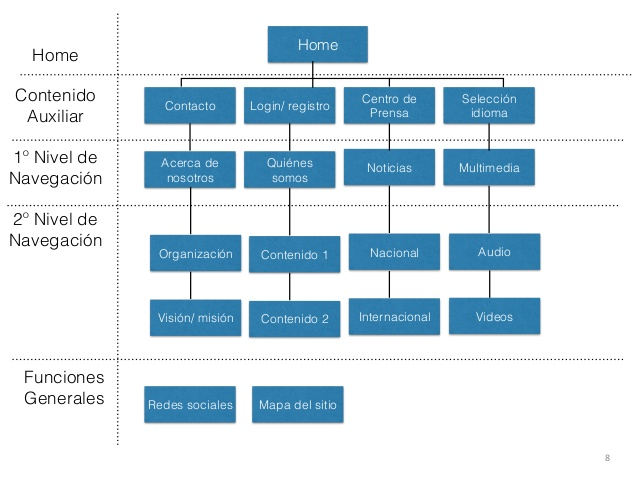
\includegraphics[width=.5\textwidth]{images/mapa}
		\caption{mapa}
		\label{fig:mapa}
	\end{center}
\end{figure}


\cdtInstrucciones{A continuación describa cada una de las pantallas.}
%% !TeX root = ../proyecto.tex
%--------------------------------------
\section{IUX Interfaz (nombre de la interfaz)}

\subsection{Objetivo}
	\cdtInstrucciones{Describa el objetivo, propósito o función de la pantalla.}

\subsection{Diseño}
	\cdtInstrucciones{Describa brevemente los elementos de la pantalla y como de be usarse a manera de manual de usuario.} Esta pantalla \IUref{IU23}{Pantalla de Control de Acceso} aparece al iniciar el sistema, para ingresar ... 

\IUfig[.7]{Login}{IU23}{Pantalla de Control de Acceso.}

%\IUfig[ancho de la figura: valor entre 1 y .1]{Nombre corto de la pantalla sin espacions ni acentos}{IUXX}{Nombre largo de la pantalla.}

\subsection{Salidas}

	\cdtInstrucciones{Liste las salidas de la interfaz. Si coinciden con las del caso de uso solo indiquelo. Esta ,ista debe incluir los mensajes}

	\begin{itemize}
		\item Descripción de salida.
	\end{itemize}
	
\subsection{Entradas}

	\cdtInstrucciones{Liste las entradas de la interfaz. Si coinciden con las del caso de uso solo indiquelo.}
	\begin{itemize}
		\item Descripción de salida.
	\end{itemize}

\subsection{Comandos}
	\cdtInstrucciones{Describa cada control (botónes, areas de drag and drop, componentes interactivos, animaciones, etc.) que se puede utilizar dentro de la pantalla indicando o que hacen y si cambia de pantalla.}

\begin{itemize}
	\item \IUbutton{Entrar}: Verifica que el Estudiante se encuentre registrado y la contraseña sea la correcta. Si la verificación es correcta, se muestra la \IUref{UI32}{Pantalla de Selección de Seminario}.
	\item \IUbutton{Ayuda}: Muestra la ayuda de esta pantalla \IUref{IU50}{Pantalla de Ayuda}.
\end{itemize}


% !TeX root = ../proyecto.tex
%--------------------------------------
\section{IU001 Interfaz (Control de acceso)}

\subsection{Objetivo}
	\cdtInstrucciones{Describa el objetivo, propósito o función de la pantalla.}
Esta Interfaz tiene como objetivo permitir al usuario introducir sus datos para acceder al sistema.
\subsection{Diseño}
	\cdtInstrucciones{Describa brevemente los elementos de la pantalla y como de be usarse a manera de manual de usuario.} 
 Esta pantalla \IUref{IU001}{Pantalla de Control de Acceso} aparece al iniciar el sistema, para ingresar su identificador tiene un cmpo de texto en la parte de arriba, un campo de contraseña para ingresar su contraseña, debajo un boton para enviar el formulario y finalmente un hipervinculo para acceder a la recuperacion de contraseña. 

\IUfig[.7]{IU001}{IU001}{Pantalla de Control de Acceso.}

%\IUfig[ancho de la figura: valor entre 1 y .1]{Nombre corto de la pantalla sin espacions ni acentos}{IUXX}{Nombre largo de la pantalla.}

\subsection{Salidas}

	\cdtInstrucciones{Liste las salidas de la interfaz. Si coinciden con las del caso de uso solo indiquelo. Esta ,ista debe incluir los mensajes}

	\begin{itemize}
		\item Coincide con el caso de uso
	\end{itemize}
	
\subsection{Entradas}

	\cdtInstrucciones{Liste las entradas de la interfaz. Si coinciden con las del caso de uso solo indiquelo.}
	\begin{itemize}
		\item Coincide con el caso de uso.
	\end{itemize}

\subsection{Comandos}
	\cdtInstrucciones{Describa cada control (botónes, areas de drag and drop, componentes interactivos, animaciones, etc.) que se puede utilizar dentro de la pantalla indicando o que hacen y si cambia de pantalla.}

\begin{itemize}
	\item \IUbutton{Entrar}: Verifica los datos del formulario esten llenos, el id exista, la contraseña coincida con la guardada y la cuenta no este suspendida, ademas busca el rol del perfil. Si la verificación es correcta, se muestra la \IUref{IU-003}{Pantalla Principal}.
	\item \IUbutton{Recuperr Contraseña}:Se muestra la \IUref{IU-004}{Recuperar contraseña}.
\end{itemize}


% !TeX root = ../proyecto.tex
%--------------------------------------
\section{IU003 Interfaz (Pagina Principal)}

\subsection{Objetivo}
	\cdtInstrucciones{Describa el objetivo, propósito o función de la pantalla.}
Esta Interfaz tiene como objetivo permitir al usuario una facil navegación a traves del sistema y las funcionalidades que el puede usar.
\subsection{Diseño}
	\cdtInstrucciones{Describa brevemente los elementos de la pantalla y como de be usarse a manera de manual de usuario.} Esta pantalla \IUref{IU003}{Pantalla Principal} aparece al acceder al sistema, consta de un menu desplegable con las siguientes categorias, nombre, materias,escuela .

\IUfig[.7]{IU003}{IU003}{Pantalla Principal.}

%\IUfig[ancho de la figura: valor entre 1 y .1]{Nombre corto de la pantalla sin espacions ni acentos}{IUXX}{Nombre largo de la pantalla.}

\subsection{Salidas}

	\cdtInstrucciones{Liste las salidas de la interfaz. Si coinciden con las del caso de uso solo indiquelo. Esta ,ista debe incluir los mensajes}

	\begin{itemize}
		\item Notificaciones
	\end{itemize}
	
\subsection{Entradas}

	\cdtInstrucciones{Liste las entradas de la interfaz. Si coinciden con las del caso de uso solo indiquelo.}
	\begin{itemize}
		\item Ninguna.
	\end{itemize}

\subsection{Comandos}
	\cdtInstrucciones{Describa cada control (botónes, areas de drag and drop, componentes interactivos, animaciones, etc.) que se puede utilizar dentro de la pantalla indicando o que hacen y si cambia de pantalla.}

\begin{itemize}
	\item \IUbutton{Entrar}: Verifica los datos del formulario esten llenos, el id exista, la contraseña coincida con la guardada y la cuenta no este suspendida, ademas busca el rol del perfil. Si la verificación es correcta, se muestra la \IUref{IU-003}{Pantalla Principal}.
	\item \IUbutton{Recuperr Contraseña}:Se muestra la \IUref{IU-004}{Recuperar contraseña}.
\end{itemize}


% !TeX root = ../proyecto.tex
%--------------------------------------
\section{IU004 Interfaz (Recuperar contraseña)}

\subsection{Objetivo}
	\cdtInstrucciones{Describa el objetivo, propósito o función de la pantalla.}
Esta Interfaz tiene como objetivo permitir al usuario recuperar su contraseña si la olvido pero recuerda su identificador y su correo.
\subsection{Diseño}
	\cdtInstrucciones{Describa brevemente los elementos de la pantalla y como de be usarse a manera de manual de usuario.} Esta pantalla \IUref{IU004}{Recuperar contraseña} contiene solo dos campos de texto y un botón para enviar el formulario .

\IUfig[.7]{IU004}{IU004}{Recuperar contraseña.}

%\IUfig[ancho de la figura: valor entre 1 y .1]{Nombre corto de la pantalla sin espacions ni acentos}{IUXX}{Nombre largo de la pantalla.}

\subsection{Salidas}

	\cdtInstrucciones{Liste las salidas de la interfaz. Si coinciden con las del caso de uso solo indiquelo. Esta ,ista debe incluir los mensajes}

	\begin{itemize}
		\item Igual al caso de uso
	\end{itemize}
	
\subsection{Entradas}

	\cdtInstrucciones{Liste las entradas de la interfaz. Si coinciden con las del caso de uso solo indiquelo.}
	\begin{itemize}
		\item Igual al caso de uso.
	\end{itemize}

\subsection{Comandos}
	\cdtInstrucciones{Describa cada control (botónes, areas de drag and drop, componentes interactivos, animaciones, etc.) que se puede utilizar dentro de la pantalla indicando o que hacen y si cambia de pantalla.}

\begin{itemize}
	\item \IUbutton{Recuperar}: Verifica los datos del formulario esten llenos, el id exista, la cuenta no este suspendida, y que el correo coincida con el guarddo. Si la verificación es correcta, se muestra la \IUref{IU-001}{Control de acceso}.
	
\end{itemize}


% !TeX root = ../proyecto.tex
%--------------------------------------
\section{IU005 Interfaz (Registro Centro de Trabajo)}

\subsection{Objetivo}
	\cdtInstrucciones{Describa el objetivo, propósito o función de la pantalla.}
 Esta Interfaz tiene como objetivo permitir al usuario introducir nuevos centros de trabajo, claves de centro de trabajo y/o prestamos de las mismas al programa.

\subsection{Diseño}
	\cdtInstrucciones{Describa brevemente los elementos de la pantalla y como de be usarse a manera de manual de usuario.} Esta pantalla \IUref{IU005}{Registro Centro de Trabajo} aparece al seleccionar la opción en el menú, contiene 5 campos de texto que deben ser llenados con los datos del Centro de trabajo, tambien tiene 2 seletores y un boton para intentar guardar los datos.
\clearpage
\IUfig[.5]{IU005}{IU005}{Registro Centro de Trabajo.}

%\IUfig[ancho de la figura: valor entre 1 y .1]{Nombre corto de la pantalla sin espacions ni acentos}{IUXX}{Nombre largo de la pantalla.}

\subsection{Salidas}

	\cdtInstrucciones{Liste las salidas de la interfaz. Si coinciden con las del caso de uso solo indiquelo. Esta ,ista debe incluir los mensajes}

	\begin{itemize}
		\item Coincide con el caso.
	\end{itemize}
	
\subsection{Entradas}

	\cdtInstrucciones{Liste las entradas de la interfaz. Si coinciden con las del caso de uso solo indiquelo.}
	\begin{itemize}
		\item Coincide con el caso.
	\end{itemize}

\subsection{Comandos}
	\cdtInstrucciones{Describa cada control (botónes, areas de drag and drop, componentes interactivos, animaciones, etc.) que se puede utilizar dentro de la pantalla indicando o que hacen y si cambia de pantalla.}

\begin{itemize}
	\item \IUbutton{Registrar}: Verifica que los datos introducidos sean validos y tengan el formato correcto, de ser asi guardara el nuevo centro de trabajo limpiando el formulario.
	
\end{itemize}


% !TeX root = ../proyecto.tex
%--------------------------------------
\section{IU006 Interfaz (registro de Salon)}

\subsection{Objetivo}
	\cdtInstrucciones{Describa el objetivo, propósito o función de la pantalla.}

\subsection{Diseño}
	\cdtInstrucciones{Describa brevemente los elementos de la pantalla y como de be usarse a manera de manual de usuario.} Esta pantalla \IUref{IU001}{Pantalla de Control de Acceso} aparece al iniciar el sistema, para ingresar ... 

\IUfig[.5]{IU006}{IU006}{Registro de salon.}

%\IUfig[ancho de la figura: valor entre 1 y .1]{Nombre corto de la pantalla sin espacions ni acentos}{IUXX}{Nombre largo de la pantalla.}

\subsection{Salidas}

	\cdtInstrucciones{Liste las salidas de la interfaz. Si coinciden con las del caso de uso solo indiquelo. Esta ,ista debe incluir los mensajes}

	\begin{itemize}
		\item Descripción de salida.
	\end{itemize}
	
\subsection{Entradas}

	\cdtInstrucciones{Liste las entradas de la interfaz. Si coinciden con las del caso de uso solo indiquelo.}
	\begin{itemize}
		\item Descripción de salida.
	\end{itemize}

\subsection{Comandos}
	\cdtInstrucciones{Describa cada control (botónes, areas de drag and drop, componentes interactivos, animaciones, etc.) que se puede utilizar dentro de la pantalla indicando o que hacen y si cambia de pantalla.}

\begin{itemize}
	\item \IUbutton{Entrar}: Verifica que el Estudiante se encuentre registrado y la contraseña sea la correcta. Si la verificación es correcta, se muestra la \IUref{UI32}{Pantalla de Selección de Seminario}.
	\item \IUbutton{Ayuda}: Muestra la ayuda de esta pantalla \IUref{IU50}{Pantalla de Ayuda}.
\end{itemize}


% !TeX root = ../proyecto.tex
%--------------------------------------
\section{IU007 Interfaz (Asignación de Director)}

\subsection{Objetivo}
	\cdtInstrucciones{Describa el objetivo, propósito o función de la pantalla.}

\subsection{Diseño}
	\cdtInstrucciones{Describa brevemente los elementos de la pantalla y como de be usarse a manera de manual de usuario.} Esta pantalla \IUref{IU007}{Asignación de Director} aparece al iniciar el sistema, para ingresar ... 

\IUfig[.7]{IU007}{IU007}{Asignación de Director.}

%\IUfig[ancho de la figura: valor entre 1 y .1]{Nombre corto de la pantalla sin espacions ni acentos}{IUXX}{Nombre largo de la pantalla.}

\subsection{Salidas}

	\cdtInstrucciones{Liste las salidas de la interfaz. Si coinciden con las del caso de uso solo indiquelo. Esta ,ista debe incluir los mensajes}

	\begin{itemize}
		\item Descripción de salida.
	\end{itemize}
	
\subsection{Entradas}

	\cdtInstrucciones{Liste las entradas de la interfaz. Si coinciden con las del caso de uso solo indiquelo.}
	\begin{itemize}
		\item Descripción de salida.
	\end{itemize}

\subsection{Comandos}
	\cdtInstrucciones{Describa cada control (botónes, areas de drag and drop, componentes interactivos, animaciones, etc.) que se puede utilizar dentro de la pantalla indicando o que hacen y si cambia de pantalla.}

\begin{itemize}
	\item \IUbutton{Entrar}: Verifica que el Estudiante se encuentre registrado y la contraseña sea la correcta. Si la verificación es correcta, se muestra la \IUref{UI32}{Pantalla de Selección de Seminario}.
	\item \IUbutton{Ayuda}: Muestra la ayuda de esta pantalla \IUref{IU50}{Pantalla de Ayuda}.
\end{itemize}


%!TEX root = ejemplo.tex
%=========================================================
\section{Catálogo de mensajes}	
\label{sec:mensajes}

	En esta sección se describen todos los mensajes que aparecen en el sistema. Para cada mensaje se especifica:
	 
	\begin{description}\itemsep0em
		\item[Id:] Identificador del mensaje de la forma ``MSG XX'' y descripción corta del mismo.
		\item[Tipo:] Tipo del mensaje el cual puede ser: 
		\begin{description}
			\item[Normal:] Mensaje que informa al usuario una instrucción o el estado interno que guarda el sistema, suele tener un color {\color{msgNormalColor}Azul}.
			\item[Éxito:] Mensaje que informa al usuario sobre una acción realizada, sirve para confirmar el correcto funcionamiento del sistema. Se presentan con un color {\color{msgInfoColor}Verde}.
			\item[Atención:] Mensaje que tiene como finalidad llamar la atención del usuario a una situación que requiere su intervención, por ejemplo cuando una actividad ha generado un efecto colateral o se realizará una acción destructiva y no reversible. Se presentan con un color {\color{msgWarningColor}Naranja}.
			\item[Error:] Mensaje que informa al usuario un fallo en en una operación o un impedimento para realizarla, por ejemplo: cuando no se puede efectuar la acción solicitada, cuando un dato falta o tiene un formato no aceptado por el sistema. Se presentan con un color {\color{msgErrorColor}Rojo}.
		\end{description}
		\item[Propósito:] Explicación del propósito del mensaje.
		\item[Redacción:] Redacción del mensaje.
		\item[Parámetros:] En caso de que el mensaje pueda variar se especifican los casos y la forma en que debe adaptarse la redacción
		\item[Ejemplos:] Ejemplos de como debe renderizarse el mensaje.
	\end{description}


\subsection{Lista de mensajes}

%msgNormalColor
%msgInfoColor
%msgWarningColor
%msgErrorColor

%Mensajes de error relacionado al inicio de secion (Origen CU-001)

\begin{cdtMessage}[msgInfoColor]{MSG-001}{Bienvenida al usuario}
	\item[Propósito:] Indicar al usuario que ha ingresado satisfactoriamente al sistema.
	\item[Redacción:] Bienvenido $<$nombre$>$ $<$Primer Apellido$>$.
	\item[Parámetros:] \hspace{1cm}
	\begin{itemize}
		\item $<$nombre$>$ \hyperlink{Usuario.nombre}{Nombre} del Usuario.
  \item $<$Primer Apellido$>$ \hyperlink{Usuario.primerApellido}{Primer Apellido} del Usuario.
	\end{itemize}
	\item[Ejemplos:] Bienvenido Juan Pérez.
\end{cdtMessage}

\begin{cdtMessage}[msgErrorColor]{MSG-002}{Usuario no registrado} 
	\item[Propósito:] Indica que el usuario ingresado no existe en el sistema.
	\item[Redacción:] El usuario $<$Identificador$>$ no se encuentra registrado.
	\item[Parámetros:] \hspace{1cm}
	\begin{itemize}
		\item $<$Identificador$>$ \hyperlink{Usuario.ID}{Identificador} del Usuario.
	\end{itemize}
	\item[Ejemplos:] El usuario 123123 no se encuentra registrado.
\end{cdtMessage}

\begin{cdtMessage}[msgErrorColor]{MSG-003}{Cuenta inactiva} 
	\item[Propósito:] Indicar al usuario que la cuenta especificada se encuentra inactiva.
	\item[Redacción:] La cuenta especificada $<$ID$>$ se encuentra inactiva.
	\item[Parámetros:] \hspace{1cm}
	\begin{itemize}
		\item $<$ID$>$ \hyperlink{Usuario.ID}{Identificador} del Usuario.
	\end{itemize}
	\item[Ejemplos:] La cuenta especificada 123123 se encuentra inactiva.
\end{cdtMessage}

\begin{cdtMessage}[msgErrorColor]{MSG-004}{Error de inicio de sesión}
	\item[Propósito:] Indica al usuario que la contraseña introducida es incorrecta.
	\item[Redacción:] La contraseña ingresada es incorrecta.
	\item[Parámetros:] No aplica.
	\item[Ejemplos:] La contraseña ingresada es incorrecta.
\end{cdtMessage}

\begin{cdtMessage}[msgErrorColor]{MSG-005}{Faltan Campos Obligatorios} 
	\item[Propósito:] Indicar al usuario que olvido agregar algún campo obligtorio.
	\item[Redacción:] El campo $<$campo$>$ es obligatorio y se encuentra vacio.
	\item[Parámetros:] \hspace{1cm}
	\begin{itemize}
		\item $<$campo$>$ de la IU.
	\end{itemize}
	\item[Ejemplos:] El campo contraseña es obligatorio y se encuentra vacio.
\end{cdtMessage}

%Mensajes de informacion no compatible con los filtros (CU002)

\begin{cdtMessage}[msgInfoColor]{MSG-006}{No se encontró información} 
	\item[Propósito:] Indicar al usuario que no existen elementos que cumplan con los filtros establecidos.
	\item[Redacción:] Ningún elemento cumple con los filtros puestos.
	\item[Parámetros:] \hspace{1cm}
	\begin{itemize}
		\item No aplica.
	\end{itemize}
	\item[Ejemplos:] Se puso de filtro un nombre de escuela que no existe, ergo no muestra ningún elemento.
\end{cdtMessage}

%Mensajes de error relacionados con tiempo (Duda de que CU de origen)
\begin{cdtMessage}[msgErrorColor]{MSG-007}{Campo con formato incorrecto} 
	\item[Propósito:] Indicar al usuario que el contenido de uno de sus campos no cumple con el formato requerido.
	\item[Redacción:] El campo $<$campo$>$ no cumple con el formato especificado, favor de corroborarlo.
	\item[Parámetros:] \hspace{1cm}
	\begin{itemize}
		\item $<$campo$>$ de la IU.
	\end{itemize}
	\item[Ejemplos:] El campo CURP no cumple con el formato especificado, favor de corroborarlo.
\end{cdtMessage}
\begin{cdtMessage}{MSG-008}{Tiempo restante para terminar un proceso} 
	\item[Propósito:] Indicar al usuario el tiempo restante para terminar una operación limitada en el tiempo como la reinscripción.
	\item[Redacción:] Quedan $<$tiempo$>$ para terminar la $<$operación$>$.
	\item[Parámetros:] \hspace{1cm}
	\begin{itemize}
		\item $<$tiempo$>$ Tiempo faltante para la operació especificando días, horas minutos y segundos.
		\item 
	\end{itemize}
	\item[Ejemplos:] \hspace{1cm}
	\begin{itemize}
		\item Quedan 45 días, 2 horas 12 minutos y 45 segundos para iniciar tu reinscripción.
		\item Quedan 2 minutos y 32 segundos para terminar tu reinscripción
	\end{itemize}
\end{cdtMessage}

\begin{cdtMessage}[msgInfoColor]{MSG-009}{Operación exitosa}
	\item[Propósito:] Informar al usuario que la operación solicitada ha sido ejecutada con éxito.
	\item[Redacción:] $<$Artículo$>$ $<$Operación$>$ del $<$Entidad$>$ $<$Identificador$>$ se realizó con éxito.
	\item[Parámetros:]\hspace{1pt}
	\begin{itemize}
		\item $<$Artículo$>$ $<$Operación$>$ se refiere a la operación realizada.
		\item $<$Entidad$>$ $<$Identificador$>$ se refiere al elemento del negocio donde recayó la operación, indicando el tipo del objeto y un dato que el usuario pueda usar para identificarlo.
	\end{itemize}
	\item[Ejemplo:] Algunos ejemplos son
	\begin{itemize}
		\item El registro del Alumno 342343 se realizó con éxito.
		\item La eliminación de la Tarea ``documentar el proceso'' se ha realizado con éxito.
	\end{itemize}
\end{cdtMessage}
\begin{cdtMessage}[msgErrorColor]{MSG-010}{Clave del Centro de Trabajo no Prestada} 
	\item[Propósito:] Indicar al usuario que la clave de centro de trabajo proporcionada no permite ser prestado.
	\item[Redacción:] La CCT proporcionada no permite ser prestada, por favor ponerse en contacto con el director del Centro de Trabajo propietario.
	\item[Parámetros:] \hspace{1cm}
	\begin{itemize}
		\item No aplica.
	\end{itemize}
	\item[Ejemplos:] La CCT proporcionada no permite ser prestada, por favor ponerse en contacto con el director del Centro de Trabajo propietario.
\end{cdtMessage}
\begin{cdtMessage}[msgInfoColor]{MSG-011}{registro exitoso}
	\item[Propósito:] Indicar al usuario que ha registrado satisfactoriamente un nuevo registro.
	\item[Redacción:] Se ha completado el registro de $<$nombre$>$ .
	\item[Parámetros:] \hspace{1cm}
	\begin{itemize}
		\item $<$nombre$>$ \hyperlink{Usuario.nombre}{Nombre} del Usuario.
	\end{itemize}
	\item[Ejemplos:] Se ha completado el registro de un Centro de Trabajo
\end{cdtMessage}
\begin{cdtMessage}[msgErrorColor]{MSG-012}{Fecha anterior a la fecha actual} 
	\item[Propósito:] Indicar al usuario que la fecha seleccionada es anterior a la fecha actual.
	\item[Redacción:] La fecha proporcionada es anterior al día de hoy por lo que no se puede admitir.
	\item[Parámetros:] \hspace{1cm}
	\begin{itemize}
		\item No aplica
	\end{itemize}
	\item[Ejemplos:]  La fecha proporcionada es anterior al día de hoy por lo que no se puede admitir.
\end{cdtMessage}


\end{document}
